\documentclass{llncs}

% Estos son los paquetes q ocupan todas las versiones del paper (normal y eprint)
\usepackage{setspace}
\usepackage{amsmath,amsfonts,amssymb,amstext}
\usepackage{mathtools}
\usepackage{latexsym,ifthen}
\usepackage{bbm,url}
\usepackage{float}
%\usepackage{bbold}
%\usepackage{amsthm}
\usepackage{bm}
\usepackage{xspace}
%\usepackage[pdftex,usenames,dvipsnames]{color}
\usepackage[usenames,dvipsnames]{color}
%\newtheorem{theorem}{Theoremh}
% \newtheorem{lemma}[theorem]{Lemma}
%\newtheorem{definition}{Definition}
%\newtheorem{example}{Example}
%\newtheorem{remark}{Remark}
%\usepackage{fullpage}
%\usepackage[margin=1.1in]{geometry}
\usepackage{tikz}
\usepackage{xspace}
\usetikzlibrary{arrows,chains,matrix,positioning,scopes,patterns}
\usepackage{authblk}
\usepackage[pdftex,pagebackref]{hyperref}
\usepackage{multirow}
\usepackage{wasysym}
%\usepackage{enumitem}
\usepackage[font=scriptsize]{caption}

% Temporal
\usepackage{soul}

%\usepackage[inline]{enumitem}
\usepackage{enumerate}
\usepackage{enumitem}
\usepackage{currfile}
\usepackage{multirow}
\usepackage{tikz}
\usepackage{tikz-qtree}
\usepackage{tikz-qtree-compat}
\usepackage{forest}
\usetikzlibrary{shapes}
\usepackage{calc}


\newcommand{\err}{\mathsf{err}}

\newcommand{\cat}{|}
\newcommand{\dsum}{/}
\newcommand{\pdsum}[2]{\mathrm{diag}(#1,#2)}

\newcommand{\sblt}{\stackrel{s}{\bullet}}

\newcommand{\algSize}{normalsize} 
%\newcommand{\algSize}{footnotesize}
\newcommand{\sfleft}{{\mathsf{left}}}
\newcommand{\sfright}{{\mathsf{right}}}

\newcommand{\ps}{\Psi({\dist_k})}
\newcommand{\psws}{{\Psi(\overline{\dist}_k)}}
\newcommand{\sps}{{\Psi_{\mathsf{spl}}(\dist_k)}}
\newcommand{\Sps}{\Psi_{\mathsf{spl}}}
\newcommand{\spsws}{{\Psi_\mathsf{spl}(\overline{\dist}_k)}}
\newcommand{\Spsws}{\Psi_\mathsf{spl}}
\newcommand{\spsmas}{\Psi_{\sfsum}(\dist_k)}
\newcommand{\Spsmas}{\Psi_{\sfsum}}
\newcommand{\spswsmas}{\Psi_{\sfsum}(\overline{\dist}_k)}
\newcommand{\Spswsmas}{\Psi_{\sfsum}}
\newcommand{\spswscomm}{{\Psi_{\mathsf{com}}(\overline{\dist}_k)}}
\newcommand{\Spswscomm}{\Psi_{\mathsf{com}}}
\newcommand{\bbb}{\bar{b}}
\newcommand{\capprox}{\overset{c}{\approx}}

\newcommand{\latexDeMierdaEstupido}{]}

\newcommand{\Comm}{\mathsf{Comm}}
\newcommand{\Com}{\mathsf{Com}}
\newcommand{\vect}{\mathbf{vec}}

\newcommand{\lef}{{\mathtt{l}}}
\newcommand{\rig}{{\mathtt{r}}}
\newcommand{\stmnt}{\mathsf{stm}}
%Commitment keys

%Log Left Commitment Key
\newcommand{\llck}{\vecb{g}}
%Log Right Commitment Key
\newcommand{\lrck}{\vecb{h}}
%Left Commitment Key
\newcommand{\lck}{[{\llck}]_1}
%Right Commitment Key
\newcommand{\rck}{[{\lrck}]_2}
\newcommand{\rcks}{[{\lrck}]_1}

%Commitement keys matrices

%Log Left Commitment Keys
\newcommand{\Llck}{\matr{G}}
%Log Right Commitment Keys
\newcommand{\Lrck}{\matr{H}}
%Left Commitment Keys
\newcommand{\Lck}{[\Llck]_1}
%Right Commitment Keys
\newcommand{\Rck}{[{\Lrck}]_2}
\newcommand{\Rcks}{[{\Lrck}]_1}

%For quadratic info \lck\rck^\top
\newcommand{\Lqmatr}{\matr{C}}
\newcommand{\Qmatr}{{[\Lqmatr]_1}}
\newcommand{\Qspace}{\mathcal{C}}

% c_\Delta
\newcommand{\lccom}{\vecb{c}_\Delta}
\newcommand{\ccom}{\hvecb{c}_\Delta}

\newcommand{\pke}{\mathsf{PKE}}
\newcommand{\kem}{\mathsf{KEM}}
\newcommand{\prf}{\mathsf{PRF}}
\newcommand{\ev}{\mathsf{F}}
\newcommand{\KEM}{\mathsf{KEM}}
\newcommand{\gen}{\mathsf{Gen}}
\newcommand{\enc}{\mathsf{Enc}}
\newcommand{\Enc}{\mathsf{Enc}}
\newcommand{\dec}{\mathsf{Dec}}
\newcommand{\Dec}{\mathsf{Dec}}
\newcommand{\pk}{\mathit{pk}}
\newcommand{\sk}{\mathit{sk}}
\newcommand{\cdh}{\ensuremath{\mathsf{CDH}}}
\newcommand{\ddh}{\ensuremath{\mathsf{DDH}}}
\newcommand{\sxdh}{\ensuremath{\mathsf{SXDH}}}
\newcommand{\mddh}{\ensuremath{\mathsf{MDDH}}}
\newcommand{\mcdh}{\ensuremath{\mathsf{MCDH}}}
\newcommand{\fmdh}{\ensuremath{\mathsf{KerMDH}}}
\newcommand{\bddh}{\ensuremath{\mathsf{BDDH}}}
\newcommand{\mat}[1]{\ensuremath{#1\mbox{-}\mathsf{Mat}}}
\newcommand{\pddh}[1]{\ensuremath{#1\mbox{-}\mathsf{PDDH}}}
\newcommand{\mlddh}[1]{\ensuremath{#1\mbox{-}\mathsf{MLDDH}}}
\newcommand{\eddh}[1]{\ensuremath{#1\mbox{-}\mathsf{EDDH}}}
\newcommand{\casc}[1]{\ensuremath{#1\mbox{-}\mathsf{Casc}}}
\newcommand{\scasc}[1]{\ensuremath{#1\mbox{-}\mathsf{SCasc}}}
\newcommand{\lin}[1]{\ensuremath{#1\mbox{-}\mathsf{Lin}}}
\newcommand{\rlin}[1]{\ensuremath{#1\mbox{-}\mathsf{RLin}}}
\newcommand{\re}{\mathsf{RE}_\G}
\newcommand{\kcirc}[1]{\ensuremath{#1\mbox{-}\mathsf{Circ}}}
\newcommand{\escQE}{\gamma}
\newcommand{\EscQE}{\Gamma}


% M \in Z^{\la \times \lb}, N\in Z^{\la \times \lc}, \Lambda\in Z^{\ld\times \lb}
% x \in \Z_q^\la, b\in \Z_q^\lb, w\in\Z_q^\lc, \alpha\in \Z_q^\ld
\newcommand{\la}{{\ell_1}}
\newcommand{\lb}{{m}}
\newcommand{\lc}{{\ell_2}}
\newcommand{\ld}{{\ell_3}}


\newcommand{\LangMN}{{\Lang_{[\matr{M}]_1,[\matr{N}]_1,\matr{\Lambda},\grkb{\alpha}}}}



\newcommand{\skermdh}{\ensuremath{\mathsf{SKerMDH}}}
\newcommand{\kermdh}{\ensuremath{\mathsf{KerMDH}}}

\newcommand{\KG}{\mathsf{KeyGen}}
\newcommand{\GS}{{\mathsf{GS}}}

%HPS definitions
\newcommand{\univo}{universal$_1$\xspace}
\newcommand{\univt}{universal$_2$\xspace}
\newcommand{\distance}[2]{\Delta\left[#1 \,,\, #2\right]}
\newcommand{\entropic}{entropic\xspace}
\newcommand{\ciphertext}{{c}}
\def\params{\mathit{params}}
\newcommand{\structure}{\mathcal{S}}
\newcommand{\ciphersp}{\mathcal{C}}
\newcommand{\conssp}{\mathcal{V}}
\newcommand{\primeorder}{p}
\newcommand{\keysp}{\mathcal{K}}
\def\hps{\varfont{hps}}
\newcommand{\advBhps}{\calB}
\newcommand{\advBhpso}{\calB_{1}}
\newcommand{\advBhpst}{\calB_{2}}
\newcommand{\PK}{\mathcal{PK}}
\newcommand{\SK}{\mathcal{SK}}
\newcommand{\hash}{\mu}
\newcommand{\bigiota}{\mathcal{I}}
\newcommand{\var}[1]{{\mathsf{#1}}}
\newcommand{\vvar}[1]{{\mathbf{\var{#1}}}}
\newcommand{\varb}{\mathsf{b}}
\newcommand{\varx}{\mathsf{x}}
\newcommand{\vvarx}{\textbf{\textsf{x}}}
\newcommand{\vary}{\mathsf{y}}
\newcommand{\vvary}{\textbf{\textsf{y}}}
\newcommand{\varz}{\mathsf{z}}
\newcommand{\varX}{\mathsf{X}}
\newcommand{\varY}{\mathsf{Y}}
\newcommand{\varZ}{\mathsf{Z}}
\newcommand{\varvecx}{\vec{\varx}}
\newcommand{\varvecy}{\vec{\vary}}
\newcommand{\varvecz}{\vec{\varx}}
\newcommand{\hcx}{(\hat{x}_1,\ldots,\hat{x}_m)}
\newcommand{\matrB}{\matr{B}} 
\newcommand{\vecL}{(\hat{l}_1,\ldots,\hat{l}_n)}



% Las instancias de SPLHS se van a llamr \Phi
\newcommand{\SPLHSinst}{\Phi}
\newcommand{\SG}{\mathsf{SignGen}}
\newcommand{\SN}{\mathsf{Sign}}
\newcommand{\SD}{\mathsf{SignDerive}}
\newcommand{\SV}{\mathsf{Verify}}
\newcommand{\SP}{\ensuremath{\mathsf{SP}}}
\newcommand{\poly}{\mathsf{poly}}

%Comicmens a los eltos de la listas
\newcommand{\lcom}{\vecb{f}}
\newcommand{\Lcom}{\matr{F}}

%Definition
\newcommand{\MP}{\mathsf{MP}}
\newcommand{\GScom}{\mathsf{GS.Com_{\hvecb{U}}}}
\newcommand{\MPcomg}{\mathsf{MP.Com}_{\hmatr{G}}}
\newcommand{\MPcomh}{\mathsf{MP.Com}_{\hmatr{H}}}




% QA-NIZK for linear spaces
\newcommand{\ZKLinInst}{\mathsf{ZKLin}}
\newcommand{\ZKLinK}{\mathsf{ZKLin.K}_0}
\newcommand{\ZKLinKK}{\mathsf{ZKLin.K}_1}
\newcommand{\ZKLinCRS}{\mathsf{ZKLin.crs}}

\newcommand{\QANIZKsum}{{\spswsmas}}
\newcommand{\QANIZKcomms}{{\spswscomm}}
\newcommand{\QANIZKsym}{{\Psi_{\mathsf{sym}}}}

\newcommand{\nb}{{\overline{n}}}

\newcommand{\bb}{\overline{b}}
\newcommand{\bub}{{b(\overline{b}-1)}}
\newcommand{\tm}{\tilde{m}}

\newcommand{\rank}{\mathbf{rank}}
\newcommand{\HPSscheme}{\mathsf{HPS}}
%\newcommand{\THPSscheme}{\schemefont{HPS_t}}
% \newcommand{\THPSscheme}{\mathsf{HPS^{td}}}
% \newcommand{\HHPSscheme}{\mathsf{HPS}_2}
\newcommand{\HPSsys}{\mathsf{Param}}
\newcommand{\HPSpub}{\mathsf{Pub}}
\newcommand{\HPSpriv}{\mathsf{Priv}}
\newcommand{\HPSdec}{\mathsf{Decide}}
\newcommand{\eval}{\Lambda}
%\newcommand{\hpscu}{{\notionfont{cu}_2}}
%\newcommand{\ExpHPScu}[2]{\Exp^{\hpscu}_{#1,#2}}
%\newcommand{\AdvHPScu}[2]{\Adv^{\hpscu}_{#1,#2}}
%\newcommand{\hpscub}{{\notionfont{\hpscu\mbox{-}b}}}
%\newcommand{\hpscuz}{{\notionfont{\hpscu\mbox{-}0}}}
%\newcommand{\hpscuo}{{\notionfont{\hpscu\mbox{-}1}}}
%\newcommand{\ExpHPScub}[2]{\Exp^{\hpscub}_{#1,#2}}
%\newcommand{\ExpHPScuo}[2]{\Exp^{\hpscuo}_{#1,#2}}
%\newcommand{\ExpHPScuz}[2]{\Exp^{\hpscuz}_{#1,#2}}
% \newcommand{\pcol}{\delta}
\newcommand{\prcol}{\delta}
\newcommand{\trapdoor}{\omega}
\newcommand{\witness}{r}
\newcommand{\algD}{\mathsf{D}}
\newcommand{\algK}{\mathsf{K}}
\newcommand{\algG}{\mathsf{G}}
\newcommand{\algP}{\mathsf{P}}
\newcommand{\algV}{\mathsf{V}}
\newcommand{\algS}{\mathsf{S}}
\newcommand{\algF}{\mathsf{F}}
\newcommand{\algVrfy}{\mathsf{Vrfy}}

\newcommand{\R}{\mathcal{R}}
\newcommand{\M}{\mathcal{M}}
\newcommand{\dist}{\mathcal{D}}
\newcommand{\distw}{\mathcal{W}}
\newcommand{\distk}{\mathcal{K}}
\newcommand{\distlin}{\mathcal{L}}
\newcommand{\distrlin}{\mathcal{RL}}
\newcommand{\distc}{\mathcal{C}}
\newcommand{\distsc}{\mathcal{SC}}
\newcommand{\distcirc}{\mathcal{CI}}
\newcommand{\distu}{\mathcal{U}}
\newcommand{\distp}{\mathcal{P}}
\newcommand{\distink}{\dist_k^{m,i}}
\newcommand{\distjnk}{\dist_1^{m,i}}

\newcommand{\distinmk}{\dist_k^{mn,i}}
\newcommand{\distzeronmk}{\dist_k^{mn,0}}
\newcommand{\distzeronk}{\dist_k^{m,0}}
\newcommand{\distlininone}{\distlin_1^{m,i}}
\newcommand{\distlinisnone}{\distlin_1^{m,i^*}}
\newcommand{\distlinizeroone}{\distlin_1^{m,0}}
\newcommand{\distlinjsnzero}{\distlin_1^{n,j^*}}
\newcommand{\block}[1]{
  \underbrace{\begin{matrix}1 & \cdots & 1\end{matrix}}_{#1}
}
%\newcommand{\gets}{\leftarrow}
\newcommand{\Z}{\mathbb{Z}}
\newcommand{\N}{\mathbb{N}}
\newcommand{\G}{\mathsf{Gen}}
\newcommand{\advD}{\mathsf{D}}
\newcommand{\advA}{\mathsf{A}}
\newcommand{\advB}{\mathsf{B}}
\newcommand{\adv}{\mathbf{Adv}}
\newcommand{\group}{{gk}}
\newcommand{\gk}{\group}
\newcommand{\pgroup}{\mathcal{PG}}
\newcommand{\mgroup}[1]{\mathcal{MG}_{#1}}
\newcommand{\ggen}{\mathsf{Gen}}
\newcommand{\pggen}{\mathsf{PGen}}
\newcommand{\mggen}[1]{\mathsf{MGen}_{#1}}
\newcommand{\heading}[1]{\smallskip\noindent{\sc{#1}}}
\newcommand{\vecb}[1]{{\boldsymbol{#1}}}
\newcommand{\vecbt}[1]{\vec{#1}^{\ \top}}
\newcommand{\uvecb}[1]{{\vect({\vecb{#1}})}}
\newcommand{\tvecb}[1]{{\tilde{\vecb{#1}}}}
\newcommand{\tgrkb}[1]{\tilde{\grkb{#1}}}
\newcommand{\ovecb}[1]{{\overline{\vecb{#1}}}}
\newcommand{\Pt}{\mathcal{P}}
\newcommand{\Opt}{\mathcal{O}}
\newcommand{\pt}[1]{\mathcal{#1}}
\newcommand{\stbl}{\ \tilde \bullet \ }
\newcommand{\bilgroup}{\mathcal{PG}}
\newcommand{\matr}[1]{\mathbf{{#1}}}
\newcommand{\vecw}{\vecb{w}}
\newcommand{\vecr}{\vecb{r}}
\newcommand{\vecz}{\vecb{z}}
\newcommand{\vecy}{\vecb{y}}
\newcommand{\vecx}{\vecb{x}}
\newcommand{\veca}{\vecb{a}}
\newcommand{\matrA}{\matr{A}}
\newcommand{\hmatrA}{\hmatr{A}}
\newcommand{\cmatrA}{\cmatr{A}}
\newcommand{\smallpmatrix}[1]{\left(\begin{smallmatrix}#1\end{smallmatrix}\right)}
\newcommand{\pmatri}[1]{\left(\begin{matrix}#1\end{matrix}\right)}
\newcommand{\bmatri}[1]{\left[\begin{matrix}#1\end{matrix}\right]}
\newcommand{\matri}[1]{{\begin{matrix}#1\end{matrix}}}
\newcommand{\smatri}[1]{{\begin{smallmatrix}#1\end{smallmatrix}}}
\newcommand{\sfsplit}{\mathsf{spl}}
\newcommand{\bulletsp}{ \bullet }
\newcommand{\newf}{\widehat{f}}
\newcommand{\newF}{\widehat{F}}
\newcommand{\com}{\mathsf{com}}
\newcommand{\eq}{\mathsf{eq}}
\newcommand{\eqd}{\equiv}
\newcommand{\negl}{\mathsf{negl}}
\newcommand{\A}{\mathcal{A}}
\newcommand{\GG}{\mathbb{G}}
\newcommand{\Gr}{\ensuremath{\mathbb{G}_1}}
\newcommand{\Hr}{\ensuremath{\mathbb{G}_2}}
\newcommand{\T}{\ensuremath{\mathbb{T}}}
\newcommand{\SSDP}{\ensuremath{\mathsf{SSDP}}}
\newcommand{\PermP}{\ensuremath{\mathsf{PermP}}}
\newcommand{\PP}{\ensuremath{\mathsf{PP^*}}}
\newcommand{\bmatr}[1]{\left[\matr{#1}\right]}
\newcommand{\hmatr}[1]{{\hat{\matr{#1}}}}
\newcommand{\cmatr}[1]{\check{\matr{#1}}}
\newcommand{\bvecb}[1]{\left[\vecb{#1}\right]}
\newcommand{\hvecb}[1]{{\hat{\vecb{#1}}}}
\newcommand{\cvecb}[1]{\check{\vecb{#1}}}
\newcommand{\bits}{\{0,1\}}
\newcommand{\rmIm}{\mathbf{Im}}
\newcommand{\sfGame}{\mathsf{Game}}
\newcommand{\sfReal}{\mathsf{Real}}
\newcommand{\grkb}[1]{{\boldsymbol #1}}
\newcommand{\ugrkb}[1]{{\underline{\grkb{#1}}}}
\newcommand{\hgrkb}[1]{\hat{\grkb{#1}}}
\newcommand{\cgrkb}[1]{\check{\grkb{#1}}}
\newcommand{\SDP}{\ensuremath{\mathsf{SDP}}}
\newcommand{\Span}{\mathbf{Span}}
\newcommand{\Group}{G}
\newcommand{\Forger}{\mathsf{F}}
\newcommand{\advSound}{\mathsf{P}^*}
\newcommand{\Lang}{\mathcal{L}}
\newcommand{\crs}{\mathsf{crs}}
\newcommand{\sfproof}{\mathsf{proof}}
\newcommand{\sfbits}{\mathsf{bits}}
\newcommand{\sfbitsn}{{\mathsf{bits},n}}
\newcommand{\sflin}{\mathsf{lin}}
\newcommand{\sfcom}{\mathsf{com}}
\newcommand{\sfbin}{\mathsf{bin}}
\newcommand{\sfset}{\mathsf{set}}
\newcommand{\sfsum}{\mathsf{sum}}
\newcommand{\rp}{{\mathsf{range}\mbox{-}\mathsf{proof}}}
\newcommand{\ovG}{\overline{\matr{G}}}
\newcommand{\ovc}{\overline{\vecb{c}}}
\newcommand{\ovb}{\overline{\vecb{b}}}

\newcommand{\dmatrix}[1]{\begin{pamtrix}#1 & \cdots & \vecb{0}\\\vdots & \ddots & \vdots\\\vecb{0}& \ldots & #1\end{pmatrix}}
\newcommand{\sdmatrix}[1]{\smallpmatrix{#1 & \cdots & \vecb{0}\\\vdots & \ddots & \vdots\\\vecb{0}& \ldots & #1}}


%weas q hay que hacer pa q no webee el latex
\newsavebox{\smlmat}% Box to store smallmatrix content
\newsavebox{\smat}
\savebox{\smlmat}{$\left(\begin{smallmatrix}
\matr{G}_1 & \ldots & \vecb{0}   & \vecb{g}_{n+1} & \ldots & \vecb{0}\\
\vdots     & \ddots & \vdots     & \vdots         & \ddots & \vdots\\
\vecb{0}   & \ldots & \matr{G}_1 & \vecb{0}       & \ldots & \vecb{g}_{n+1}
\end{smallmatrix}\right)$}

\savebox{\smat}{$\left(\begin{matrix}
s_1 & \ldots & s_n\\
0   & \ldots & 0
\end{matrix}\right)$}






\newcommand{\sG}{|\GG_1|}
\newcommand{\sH}{|\GG_2|}
\newcommand{\s}{(\sG+\sH)}

\newcommand{\vu}{\hat{\vecb{u}}}
%\newcommand{\vv}{\check{\vecb{v}}}
\newcommand{\vc}{\hat{\vecb{c}}}
\newcommand{\vd}{\check{\vecb{d}}}
\newcommand{\zip}{\mathbf{zip}}

\newcommand{\indexSet}[2]{\mathcal{I}_{#1,#2}}
\newcommand{\SignaturesSet}{\mathcal{S}}
\newcommand{\Sign}{\mathsf{Sign}}
\newcommand{\Ver}{\mathsf{Ver}}

\newcommand{\bit}{\mathsf{bit}}
\newcommand{\sfts}{\mathsf{ts}}

%El-Gamal keys
\newcommand{\egpk}{\hat{x}}
\newcommand{\egsk}{x}
\newcommand{\egvpk}{\hvecb{k}}
\newcommand{\egvsk}{\vecb{k}}

%The set of permutation matrices
\newcommand{\matrPerms}{\mathcal{S}}
%The set of permutations
\newcommand{\Perms}{S}

\newcommand{\duda}[1]{{\iffalse\color{red}#1\fi}}

\newcommand{\cambio}[2]{{\iffalse\color{blue}Ahora: \fi#1}{\iffalse\color{red}(Antes: #2)\fi}}

\newenvironment{code}
   {\begin{tabbing}
   \hspace{4mm} \= \hspace{4mm} \= \hspace{4mm} \= \hspace{4mm} \= \hspace{4mm} \= \kill \\
   }
   {\end{tabbing}}

%\newcommand{\authnote}[2]{\medskip \noindent {\bf #1 says:} #2}
\newcommand{\authnote}[2]{\medskip \noindent {\bf #1 says:} {\textcolor{blue}{#2}}}

%\newtheorem{corollary}{Corollary}

\newtheorem{fact}{Fact}
\newtheorem{observation}{Observation}

\newcommand{\Am}{A}
\newcommand{\vX}{\ensuremath{\hat{\vecb{x}}}}
\newcommand{\VX}{\ensuremath{\hat{\vecb{v}}}}
\newcommand{\WX}{\ensuremath{\hat{\vecb{w}}}}
\newcommand{\VY}{\ensuremath{\check{\vecb{v}}}}
\newcommand{\WY}{\ensuremath{\check{\vecb{w}}}}
\newcommand{\vy}{\ensuremath{\vecb{y}}}
\newcommand{\vY}{\ensuremath{\check{\vecb{y}}}}
\newcommand{\vx}{\ensuremath{\vecb{x}}}


\newcommand{\U}{\ensuremath{\vecb{u}}}
\newcommand{\V}{\ensuremath{\vecb{v}}}
\newcommand{\vr}{\ensuremath{\vecb{r}}}
\newcommand{\vs}{\ensuremath{\vecb{s}}}
\newcommand{\vt}{\ensuremath{\vecb{t}}}


\newcommand{\ux}{\ensuremath{\hat{\vecb{u}}}}
\newcommand{\uy}{\ensuremath{\check{\vecb{u}}}}

\newcommand{\minitbl}[2]{\begin{tabular}{l}{#1}\\{#2}\end{tabular}}

\newcommand{\ef}{\iffalse}
%
%\makeatletter
%\newcommand*{\inlineequation}[2][]{%
%  \begingroup
%    % Put \refstepcounter at the beginning, because
%    % package `hyperref' sets the anchor here.
%    \refstepcounter{equation}%
%    \ifx\\#1\\%
%    \else
%      \label{#1}%
%    \fi
%    % prevent line breaks inside equation
%    \relpenalty=10000 %
%    \binoppenalty=10000 %
%    \ensuremath{%
%      % \displaystyle % larger fractions, ...
%      #2%
%    }%
%    ~\@eqnnum
%  \endgroup
%}
%\makeatother
%
%\makeatletter
%\renewcommand*{\@opargbegintheorem}[3]{\trivlist
%  \item[\hskip \labelsep{\bfseries #1\ #2}] \textbf{(#3)}\ \itshape}
%\makeatother



\author{Alonso Gonz\'alez \inst{1}}
\institute{Mi casita}

\title{Efficient NIZK for NP without Knowledge Assumptions}
\begin{document}
%\begin{doublespace}

\maketitle
\begin{abstract}
    Insert abstract here.

\end{abstract} 

\section{NIZK for NC}

	% !TEX root = ./main-circuit-nizk.tex

We construct a NIZK proof system for NC, that is circuits of polylogarithmic depth, whose proof consists of a perfectly binding commitment to the circuit inputs plus a proof that the circuit outputs 1 when evaluated in the committed inputs. The size of the proof is linear in the depth of the circuit. 

We setup a CRS composed of commitment keys indexed by a level in the circuit and labeled as L (left), R (right), and O (output). Specifically, these commitment keys are random matrices $[\matr{L}_i]_1,[\matr{R}_i]_2,[\matr{O}_1]_1,\ldots,[\matr{L}_d]_1,[\matr{R}_d]_2,[\matr{O}_d]_1$ of size $2\times(n_i+1),2\times(n_i+1),2\times(n_i+1)$, where $i\in[d]$ and $d$ is the depth of the circuit. Each commitment key is used for computing commitments of the left, right and output wires of all the gates at some given level.  Denote by $[\vecb{a}_i]_1,[\vecb{b}_i]_2,[\vecb{c}_i]_1$, $i\in[d]$, these commitments.

We compile any circuit into another circuit consisting of $d$ sets of NAND gates, each set of size $n_i$, and a set of ``wiring'' matrices $\matr{W}^L_1,\matr{W}^R_1\in\bits^{n_2\times n_{1}},\allowbreak,\ldots,\allowbreak\matr{W}^R_d\in\bits^{n_d\times n_{d-1}}$. Let $\vecb{z}_{i-1}\in\bits^{n_i-1}$ the vector of outputs at level $i$. The wiring matrices $\matr{W}^L_i$ and $\matr{W}^R_i$ are chosen such that
$$
\vecb{x}_i = \matr{W}^L_i\vecb{z}_{i-1} \text{ and } \vecb{y}_i = \matr{W}^R_i\vecb{z}_{i-1}
$$
and each row of both $\matr{W}^L_i$ and $\matr{W}^R_i$ contains at most one $1$.


For each tuple $([\vecb{c}_{i-1}]_1,[\vecb{a}_i]_1,[\vecb{b}_i]_2)$ one needs to give two proofs: a) ``correct wiring'', that is show that the input of the left and right wires at level $i$ are correctly taken from the outputs of level $i-1$; and b) a proof that $\vecb{z}_i=\mathrm{NAND}(\vecb{x}_i,\vecb{y}_i)$, where NAND is computed component-wise.

To prove``correct wiring'' of the openings of $[\vecb{c}_{i-1}]_1,[\vecb{a}_i]_1,[\vecb{b}_i]_2$ we give QA-NIZK proof of the existence of $\vecb{z}_{i-1},\vecb{\tau}_{i-1},\vecb{\rho}_i,\vecb{\sigma}_i$ such that
$$
\begin{pmatrix}
\vecb{c}_{i-1} \\ \vecb{a}_i \\ \vecb{b}_i
\end{pmatrix}
=
\begin{pmatrix}
\matr{O}^1_{i-1}  & \matr{O}^2_1  & \vecb{0}       & \vecb{0}\\
\matr{L}^1_i\matr{W}^L_i         & \vecb{0}         & \matr{L}^2_i & \vecb{0} \\
\matr{R}^1_i\matr{W}^R_i         & \vecb{0}         & \vecb{0}      & \matr{R}^2_i
\end{pmatrix}
\begin{pmatrix}
\vecb{z}_{i-1} \\ \vecb{\tau}_{i-1} \\ \vecb{\rho}_i \\ \vecb{\sigma}_i
\end{pmatrix}
$$

For the second proof, we can equivalently express it as
$$
\vecb{z}_i = \vecb{1} - \vecb{x}_i\circ\vecb{y}_i,
$$
assuming that the circuit input is a vector in $\bits^{n_0}$, which can be proven adapting QA-NIZK proofs for bitstrings. Specifically, we compute and $[\vecb{\pi}]_1\in\GG_1^4$ such that\footnote{As it is, this proof is not zero-knowledge. However, it can be easily made zero-knowledge giving two shares  of $\vecb{\pi}_i$ (one in each group) as we did in our AC paper.}
$$
\sum_{j=1}^{n_i} \vecb{\lambda}_j\otimes \vecb{\rho}_j-\vecb{a}_i\otimes\vecb{b}_i = \vecb{\pi}_i,$$  where $\vecb{\lambda}_j,\vecb{\rho}_j$ are the columns of $\matr{L}_i$ and $\matr{R}_i$, and a proof of existence of $\vecb{w}\in\Z_q^{(n_i+1)^2}$ such that
$$
\begin{pmatrix}
\vecb{\pi}_i \\ \vecb{c}_i
\end{pmatrix}
=
\begin{pmatrix}
\matr{L}^1_i\otimes\matr{R}^1_i & \matr{L}^1_i\otimes\matr{R}^2_i & \matr{L}^2_i\otimes\matr{R}^1_i & \matr{L}^2_i\otimes\matr{R}^2_i  & \vecb{0 }\\
\matr{D}_i                  & \vecb{0}                                       & \vecb{0}                                       & \vecb{0}
                                   & \matr{O}^2_i   
\end{pmatrix}
\vecb{w},
$$
where $\matr{D}_i$ are the rows of an identity matrix of size $n_i$ whose $i$ th 1 is replaced by $\vecb{o}_i$ and zeros by $\vecb{0}\in\Z_q^2$. That is
$$
\matr{D}_i := 
\begin{pmatrix}
	\vecb{o}_1\ \vecb{0}\cdots\vecb{0} |
	\vecb{0}\ \vecb{o}_2\ \vecb{0}\cdots\vecb{0} |
	\cdots |
	\vecb{0}\cdots\vecb{0}\ \vecb{o}_{n_i}
\end{pmatrix}
\in\Z_q^{n_i^2}
$$
Finally, we compute a proof that $\vecb{c}_d$ opens to 1.
\paragraph{Soundness Intuition.} Let $[\vecb{c}]_1$ the perfectly binding commitment to the circuit inputs, and assume that we are able to extract its opening $\vecb{z}_0\in\bits^{n_0}$ (which can be easily done with a constant-size proof that each opening is a bit). From $\vecb{z}_0$ we can compute an honest wire evaluation $\vecb{x}_1,\vecb{y}_1,\vecb{z}_1,\ldots,\vecb{x}_d,\vecb{y}_d,\vecb{z}_d$.

We will change the commitment keys in an computationally indistinguishable fashion, so that, at each level, commitments are perfectly binding for a single gate. Additionally, we will require that, if the commitment keys at level $i$ are perfectly binding for gate $j$, then the commitment keys at level $i-1$ are perfectly binding for some gate whose output is one of the inputs of gate $j$. Thereby, we are choosing a random path from the circuit output to one of its inputs. It will hold that for all the wires in the path the NIZK proofs will be sound (and in the other gates they will be trivially sound since the commitments are perfectly hiding).

%In order to break the binding property of commitment $\vecb{c}_0$, 
We are going to pick a path that differs at all the output wires from the corresponding honestly evaluated path. Note that if this is the case, we can extract two different openings for $\vecb{c}_0$ at the coordinate that is perfectly binding.

Consider the (unique) opening of commitments $([\vecb{a}_1]_1,\allowbreak [\vecb{b}_1]_2,\allowbreak[\vecb{c}_1]_1),\ldots,([\vecb{a}_d]_1,\allowbreak[\vecb{b}_d]_2,[\vecb{c}_d]_1)$ at the chosen path and the corresponding honestly evaluated path, say at gates $j_1,\ldots,j_d$ (note that $j_d=1$ since there is a single gate at the deepest level). We write, respectively, the former and later paths as
\begin{align*}
&(x^*_{1},y^*_{1},z^*_{1}),\ldots,(x^*_{d},y^*_{d},z^*_{d}),\\
&(x_{1,j_1},y_{1,j_1},z_{1,j_1}),\ldots,(x_{d,j_d},y_{d,j_d},z_{d,j_d}).
\end{align*}
Note that, if the adversary produces a convincing proof, then it must hold that $z^*_{d}=1$. On the other hand, for an honest evaluation it must hold that $z_{d,j_d}=0$, since otherwise the adversary is not cheating.
At this point we have $z^*_{d}\neq z_{d,j_d}$ and thus both paths differs at its last output wires. Next, we will show that this will happen for all the other output wires with non negligible probability.

Assume that $z^*_{i}\neq z_{i,j_i}$ with probability $p$. We want to show that, with probability essentially $p/2$, it also holds that $z^*_{i-1}\neq z_{i-1,j_{i-1}}$. The hypothesis implies that at that at least one of the following inequalities hold:
$$x^*_{i}\neq x_{i,j_i}\text{ or }y^*_{i}\neq y_{i,j_i}.$$ 
Indeed, by soundness of the NIZK proofs for NAND, otherwise we get that
$$z^*_{i} = \mathrm{NAND}(x^*_{i},y^*_{i})  = \mathrm{NAND}(x_{i,j_i},y_{i,j_i})=z_{i,j_i},$$
which is in fact the negation of the hypothesis. 

Now we use the fact that commitment keys at level $i-1$ are perfectly binding at a randomly chosen gate among the two whose outputs are wired to $x^*_{i,j_i}$ or $y^*_{i,j_i}$. Since with probability $1/2$ either $z^*_{i-1}=x^*_{i}$ or $z^*_{i-1}=y^*_{i}$, and $z_{i-1,j_{i-1}}=x_{i,j_i}$ or $z_{i-1,j_{i-1}}=x_{i,j_i}$, we get that, conditioned on $z^*_{i}\neq z_{i,j_i}$, $z^*_{i-1}\neq z_{i-1,j_{i-1}}$ holds with probability at least 1/2. We conclude that 
$$
\Pr[z^*_{i-1}\neq z_{i-1,j_{i-1}}] \geq \Pr[z^*_{i-1}\neq z_{i-1,j_{i-1}}|z^*_{i}\neq z_{i,j_i}]\Pr[z^*_{i}\neq z_{i,j_i}] = p/2.
$$

Using the same argument $d$ times, we can get two different openings for one of the input commitments with probability roughly $1/2^d$. Assuming $d=\mathrm{polylog}(n)$, we have that this probability is non-negligible.
	
	\subsection{The protocol}
	
		% !TEX root = ./main-circuit-nizk.tex

Consider the distributions $\dist_0,\dist_1,\ldots,\dist_n$ over matrices $\matr{U}_0,\matr{U}_1,\ldots,\matr{U}_n\in\Z_q^{2\times(n_i+1)}$ such that 
\begin{align}
\matr{U}_0 := \vecb{u}\matr{T}_2 \text{ and } \matr{U}_i := (\vecb{u}\matr{T}_1|\vecb{t}|\vecb{u}\matr{T}_2),
\end{align}
where $\matr{T}_1 \gets\Z_q^{2\times i},\matr{T}_2\gets\Z_q^{2\times(n_i+1-i)}$, $\vecb{a}\gets\Z_q^2$, and $\vecb{t}$ is chosen uniformly from $\Z_q^{2}\setminus\mathrm{Im}(\vecb{a})$.
Consider also a circuit $C$ of depth $d$ constructed from wiring matrices $\matr{W}^L_i,\matr{W}^R_i\in\bits^{n_{i+1}\times n_i}$ and NAND gates, where $i\in[d]$ and $n_0,\ldots,n_d$ are the number of inputs at levels $0,1,\ldots,d$.

Our proof system is defined as follows.
\begin{description}
\item[{$\algK_0(gk)$}:] Pick $\matr{U}\gets\dist$ and define $ck_0 := [\matr{U}]_1$, such that $ck_0$ defines perfectly binding commitments. Define $\crs_0 := ck_0$
\item[{$\algK_1(\crs_0, C)$}:]
For each $i\in[d]$,
pick $\matr{L}_i,\matr{R}_i,\matr{O}_i\gets\dist_0$ and define $ck^{L}_i := [\matr{L}_i]_1,ck^{R}_i := [\matr{R}_i]_2,ck^O_i:=[\matr{O}_i]_1$. Pick also $\crs^\mathsf{wires}_i,\crs^\mathsf{gates}_i$ for computing QA-NIZK proofs of, respectively, membership in the immage of
\begin{equation}
\matr{\Gamma}_i :=
\begin{pmatrix}
\matr{O}^1_{i-1}  & \matr{O}^2_{i-1}  & \vecb{0}       & \vecb{0}\\
\matr{L}^1_i\matr{W}^L_i         & \vecb{0}         & \matr{L}^2_i & \vecb{0} \\
\matr{R}^1_i\matr{W}^R_i         & \vecb{0}         & \vecb{0}      & \matr{R}^2_i
\end{pmatrix}\in\Z_q^{6\times (n_{i-1}+3)},
\end{equation}
where $\matr{O}_0 := \matr{U}$ and $\matr{L}_i,\matr{R}_i,\matr{O}_i$ are parsed as $\matr{L}^1_i,\matr{R}^1_i,\matr{O}^1_i\in\Z_q^{2\times n_i}$ and $\matr{L}^2_i,\matr{R}^2_i,\matr{O}^2_i\in\Z_q^{2\times 1}$, and satisfiability of the set of equations
\begin{equation}
\vecb{z}_i = \vecb{1} - \vecb{x}_i\circ\vecb{y}_i,\quad \vecb{x}_i,\vecb{y}_i,\vecb{z}_i\in\Z_q^{n_i}.
\end{equation}
Pick also $\crs^\mathsf{out}$ for proving that commitments computed with commitment key $ck_d^O$ open to one.

The CRS is
$$\crs := (gk,ck_0,\{ck^L_i,ck^R_i,ck^O_i,\crs^\mathsf{wires}_i,\crs^\mathsf{gates}_i:i\in[d]\},\crs^\mathsf{out})$$

\item[{$\algP(\mathsf{crs}, C, \vecb{z}_0)$}:]
On input $\vecb{z}_0$ such that $C(\vecb{z}_0)=1$, compute $[\vecb{c}_0]:=\Com_{ck_0^O}(\vecb{z}_0;\tau_0)$, for $\tau_0\gets\Z_q$. For each $i\in[d]$, the prover computes
$$
\vecb{x}_{i} = \matr{W}^L_{i}\vecb{z}_{i-1},\ \vecb{y}_{i} = \matr{W}^R_{i}\vecb{z}_{i-1},\text{ and }\vecb{z}_i = \mathrm{NAND}(\vecb{x}_i,\vecb{y}_i)
$$
computes commitments
\begin{align*}
[\vecb{a}_i]_1 = \mathsf{Com}_{ck_i^L}(\vecb{x}_i;\rho_i),\ 
[\vecb{b}_i]_2 = \mathsf{Com}_{ck_i^R}(\vecb{y}_i;\sigma_i),\ 
[\vecb{c}_i]_1 = \mathsf{Com}_{ck_i^O}(\vecb{z}_i;\tau_i),
\end{align*}
where $\rho_i,\sigma_i,\tau_i\gets\Z_q^r$, and proofs
\begin{align*}
&\pi_i^\mathsf{wires}\gets\Pi_\mathsf{lin}.\algP(\crs_i^\mathsf{wires},[\vecb{c}_{i-1}]_1,[\vecb{a}_i]_1,[\vecb{b}_i]_2,\vecb{z}_{i-1},\tau_{i-1},\rho_i,\sigma_i),\\
&\pi_i^\mathsf{gates}\gets\Pi_\mathsf{quad}.\algP(\crs_i^\mathsf{gates},[\vecb{c}_{i}]_1,[\vecb{a}_i]_1,[\vecb{b}_i]_2,\vecb{x}_i,\vecb{y}_i,\tau_{i},\rho_i,\sigma_i).
\end{align*}
Finally, it computes the proof
\begin{align*}
&\pi^{\mathsf{out}} \gets \Pi_\sflin.\algP(\crs^\mathsf{out}, [\vecb{c}_d]_1,\tau_d).
\end{align*}
The proof is
$$\pi:=([\vecb{c}_0]_1,\{[\vecb{a}_i]_1,[\vecb{b}_i]_2,[\vecb{c}_i]_1,\pi^\mathsf{wires}_i,\pi^\mathsf{gates}_i:i\in[d]\},\pi^\mathsf{out}).$$
\item[{\(\algV(\crs,C,\pi)\)}:]
Parse $\pi$ as $([\vecb{c}_0]_1,\{[\vecb{a}_i]_1,[\vecb{b}_i]_2,[\vecb{c}_i]_1,\pi^\mathsf{wires}_i,\pi^\mathsf{gates}_i:i\in[d]\},\pi^\mathsf{out})$ and check the validity of each of the proofs. Return 0 if any of the ckecks fails, else return 1.

\item[$\mathsf{S}_1$:] TBD.

\item[$\mathsf{S}_2$:] TBD.
\end{description}

We prove the following Theorem.

\begin{theorem} \label{theo:bits}
The proof system described above is a composable NIZK AoK proof system for the language \(\mathsf{CircuitSat}(C)\)
 with perfect completeness, computational soundness, and perfect zero-knowledge.
\end{theorem}	
Perfect completeness follows directly by inspection.
For proving perfect soundness we consider the extractor $\algE$ which, given the commitment $[\vecb{c}_0]_1$ and a trapdoor $\tau$, it outputs the opening $\vecb{z}_0\in\bits^{n_0}$. (Here we are assuming that $\vecb{c}_0$ is extractable in $\bits^{n_0}$)

Computational knowledge soundness follows from the indistinguishability of the following games:
\begin{description}
\item[$\sfReal$:] This is the real game. The adversary wins if $\advA||\algE$ outputs $((C,\pi),\vecb{z}_0)$ such that $C(\vecb{z}_0)=0$ and $\algV(\crs,C,\pi)=1$.
\item[$\sfGame_{1}$] This game is exactly $\sfReal$ except that the extractor is run to compute an opening $\vecb{z}_0$ of $[\vecb{c}_0]_1$, and an honest evaluation of the wires $\vecb{x}_i,\vecb{y}_i,\vecb{z}_i$, $i\in[d]$, is computed from $\vecb{z}_0$. Define also $j_d\gets 1$ and $\mathsf{label}_d \gets \perp$.
\item[$\sfGame_{1,i}$:] For $i=d$ to $1$, this game is exactly as $\sfGame_{3,i+1}$ except that picks the commitments keys for level $i$ from the distribution $\dist_{j_i}$. {\color{red} Note that in this game there are a unique openings $x^*_i,y^*_i,z^*_i$ and randomness $\rho^*_,\sigma^*_i,\tau^*_i$ such that $\vecb{a}_i = x^*_i\vecb{t}+\rho^*_i\vecb{u}, \vecb{b}_i = y^*_i\vecb{t}+\sigma^*_i\vecb{u}, \vecb{c}_i = z^*_i\vecb{t}+\tau^*_i\vecb{u}$, and the same happens for all deeper levels.}

\item[$\sfGame_{2,i}$:] For $i=d$ to $1$, this game is exactly as $\sfGame_{1,i}$ except that it  aborts if any of the following conditions hold:
\begin{itemize}
 	\item[$E_1$ :] $z^*_{i}= z_{i,j_i}$,
 	\item[$E_2$ :] $z^*_i\neq \mathrm{NAND}(x^*_i,y^*_i)$.
 	\item[$E_3$ :] $\mathsf{label}_i = L$ and $z^*_i \neq x^*_{i+1}$,
 	\item[$E_4$ :] $\mathsf{label}_i = R$ and $z^*_i \neq y^*_{i+1}$.
\end{itemize}

\item[$\sfGame_{3,i}$:] For $i=d$ to $1$, this game is exactly as $\sfGame_{2,i}$ with the following modifications. An additional label $\mathsf{label}_i$ is randomly is chosen from $\{L,R\}$, and $j_{i-1}$ is defined as the index of the gate at level $i-1$ connected to the left or right wire if, respectively, $\mathsf{label}_i = L$ or $\mathsf{label}_i = R$. Additionally the game aborts if any of the following conditions hold:
\begin{itemize}
	\item[$E_5$ :] $\mathsf{label}_i=L$ and $x^*_i = x_{i,j_i}$,
	\item[$E_6$ :] $\mathsf{label}_i=R$ and $y^*_i = y_{i,j_i}$.
\end{itemize}
\end{description}
 
%\begin{theorem} Let \(\mathsf{Adv}_{{\Pi_\sfset}}(\advA)\) 
%be the advantage of an adversary \(\advA\) against the soundness of 
%the proof system  described above. There exist PPT adversaries
%\(\advD_1,\advD_2,\advB_\sfbits,\advB_\sfcom,\advB_\sfsum,\advB_\mathsf{lin}\) such that 
%\begin{align*}
%\mathsf{Adv}_{{\Pi_\sfset}}(\advA) \leq 
%n \left(\right.
%    &\mathsf{Adv}_{\mathcal{L}_1,\Gr}(\advD_1) 
%        + \setsize /2\left(4/q
%            +  \mathsf{Adv}_{\Pi_\sfbits}(\advB_\sfbits)
%            +  \mathsf{Adv}_{\mathcal{L}_1,\Hr}(\advB_2)\right. \\
%    &+ \left.\left.\mathsf{Adv}_{{\Pi_\sfcom}}(\advB_\sfcom)
%        + m\mathsf{Adv}_{{\Pi_\sfsum}}(\advB_\sfsum)
%        + m\mathsf{Adv}_{{\Pi_\mathsf{lin}}}(\advB_\mathsf{lin})\right)\right).
%\end{align*}
%\label{teo:bitstr-soundness}
%\end{theorem}

It is obvious that the first two games are indistinguishable. We define $\sfGame_{3,d+1}\equiv\sfGame_1$. The sequence of games is
$$
\mathsf{Real}  \to \sfGame_1 \equiv \sfGame_{3,d+1} \to \sfGame_{1,d} \to \ldots \sfGame_{3,d}\to \sfGame_{1,d-1}\to
\ldots \to \sfGame_{3,1}
$$
The rest of the argument goes follows from the following lemmas.

\begin{lemma} \label{lemma:3-1}
For any $i\in[d]$ and any PPT $\advA$ there exists PPT $\advB_1,\advB_2$ such that 
$$|\Pr\left[ \mathsf{Game}_{3,i+1}(\advA)=1\right]-\Pr\left[ \mathsf{Game}_{1,i}(\advA)=1\right]|\leq 2\adv_{\mathrm{DDH},\GG_1}(\advB_1)+\adv_{\mathrm{DDH},\GG_2}(\advB_2).$$
\end{lemma}

\begin{proof}  Direct no?
\end{proof}

\begin{lemma} \label{lemma:1-2}
For any $i\in[d]$ and any PPT $\advA$ there exists PPT $\advB_1,\advB_2$ such that 
$$|\Pr\left[ \mathsf{Game}_{1,i}(\advA)=1\right]-\Pr\left[ \mathsf{Game}_{2,i}(\advA)=1\right]|\leq 2\adv_{\Pi_\mathsf{lin}}(\advB_1)+\adv_{\Pi_\mathsf{quad}}(\advB_2).$$
\end{lemma}

\begin{proof}  Note that the difference between the adversary advantage if both games is upper bounded by $\Pr[E_1]+\Pr[E_2]+\Pr[E_3\cup E_4]$. We proceed to bound these probabilities

\begin{description}
\item[$E_1$ :]
By induction on $i$, with base case $i=d$ and inductive step that goes from $i+1$ to $i$, we prove that $\Pr[E_1]\leq \adv_{\Pi_\mathsf{lin}}(\advB_1)$ for some PPT $\advB_1$. Note that with probability at least $\Pr[\adv_{\Pi_\mathsf{lin}}(\advB_1)]$ we have that $z^*_{d,} = 1$, since otherwise we can build $\advB_2$ that breaks soundness of the proof that $\vecb{c}_d$ opens to 1. On the other hand if $\sfGame_{1,i}(\advA)=1$ then $C(\vecb{z}_0)z_{d,j_d}=0$. We conclude that $\Pr[E_1]\leq \adv_{\Pi_\mathsf{lin}}(\advB_1)$.

Assume now that $z^*_{i+1}\neq z_{i+1,j_{i+1}}$. Without loss of generality, assume $\mathsf{label}_i = L$ (the other case is similar).
Since otherwise $\sfGame_{2,i+1}$ would have aborted (and hence also $\sfGame_{1,i}$ would have aborted), it holds that $z^*_i = x^*_{i+1}$. Similarly, since otherwise $\sfGame_{3,i+1}$ would have aborted, $x^*_{i+1} \neq x_{i+1,j_{i+1}}$. It follows that $z^*_i \neq x_{i+1,j_{i+1}}=z_{i,j_i}$ and hence $\Pr[E_1]=0$.

\item[$E_2$ :] Clearly, if $z^*_i \neq \mathrm{NAND}(x^*_i,y^*_i)$ then we can build an adversary $\advB_2$ against $\Pi_\mathsf{quad}$. Therefore, $\Pr[E_2]\leq \adv_{\Pi_\mathsf{quad}}(\advB_2)$.

\item[$E_3\cup E_4$ :] Without loss of generality, assume that $\mathsf{label}_i = L$ (the other case is symmetric).
The fact that $\vecb{c}_i$ is perfectly binding at coordinate $j_i$ implies that every solution to $\vecb{c}_i/\vecb{a}_{i+1}/\vecb{b}_{i+1} \in \matr{\Gamma}_{i+1}\vecb{w}$ is equal to $z^*_i$ at position $j_i$.\footnote{Here `/' means vertical concatenation.}
Since $\mathsf{label}_i = L$, then the $j_{i+1}$ row of $\matr{W}_{i+1}^L$ is equal to $\vecb{e}^\top_{j_i}$ --- meaning that the output of gate $j_{i+1}$ is connected to the left input of gate $j_i$.
Then
$$
\vecb{a}_{i+1} = 
	(\vecb{a}\matr{T}_1|\vecb{t}|\vecb{a}\matr{T}_2)\pmatri{\matr{W}^R_{i+1}|\vecb{0}\\0\cdots 0|1}\pmatri{\vecb{w}\\\rho^*_i} =
	\vecb{e}_{j_i}^\top\vecb{w}\vecb{t}+ \rho^*_i\vecb{a} = z_i^*\vecb{t}+\tilde{\rho}_i\vecb{a},
$$
for some $\tilde{\rho}_i\in\Z_q$.

Since $\vecb{a}_{i+1}$ is perfectly binding at coordinate $j_{i+1}$, we get that $z^*_i = x^*_{i+1}$. Thus, $z^*_i \neq x^*_{i+1}$ implies that $\vecb{c}_i/\vecb{a}_{i+1}/\vecb{b}_{i+1} \notin \mathrm{Im}(\matr{\Gamma}_{i+1})$ and we can construct an adversary $\advB_1$ such that $\Pr[E_3\cup E_4] \leq \adv_{\Pi_\mathsf{lin}}(\advB_1)$.
\end{description}
\end{proof}

\begin{lemma} \label{lemma:2-3}
For any $i\in[d]$ it holds that,  
$$\Pr\left[ \mathsf{Game}_{2,i}(\advA)=1\right]\leq 2\Pr\left[ \mathsf{Game}_{3,i}(\advA)=1\right].$$
\end{lemma}
\begin{proof}
Since $\sfGame_{2,i}$ return 1 only if $z^*_i \neq z_{i,j_i}$, it must be that
$$
z^*_i = \mathrm{NAND}(x^*_i,y^*_i) \neq \mathrm{NAND}(x_{i,j_i},y_{i,j_i}) = z_{i,j_i}
$$
and hence, conditioned on $\sfGame_{2,i}(\advA)=1$, at least one of $x^*_i\neq x_{i,j_i}$ or $y^*_i\neq y_{i,j_i}$ holds. This in turn implies that
$$
\Pr[y^*_i = y_{i,{j_i}}|\sfGame_{2,i}(\advA)=1] \leq \Pr[x^*_i \neq x_{i,{j_i}}|\sfGame_{2,i}(\advA)=1].
$$
Since $\mathsf{label}_i$ remains information theoretically hidden to the adversary and is thus independent of $x^*_i,y^*_i,x_{i,j_i},y_{i,j_i}$, it follows that
\begin{align*}
&\Pr[E_5] = \Pr[\{\mathsf{label}_i = L\} \cap \{x^*_i = x_{i,{j_i}}\}] = \frac{1}{2}\Pr[x^*_i = x_{i,{j_i}}]\\
&\Pr[E_6] = \Pr[\{\mathsf{label}_i = R\} \cap \{y^*_i = y_{i,{j_i}}\}] \leq \frac{1}{2}\Pr[x^*_i \neq x_{i,{j_i}}]\\
\Longrightarrow
& \Pr[\overline{E_5\cup E_6}] \geq 1 - (\Pr[E_5]+\Pr[E_6]) \geq 1-1/2=1/2,
\end{align*}
where all probabilities are taken conditioned on $\sfGame_{2,i}(\advA)=1$.
We conclude that
\begin{align*}
\Pr[\sfGame_{3,i}(\advA)] &\geq \Pr[\sfGame_{3,i}(\advA)=1|\overline{E_5\cup E_6}]\Pr[\overline{E_5\cup E_6}] \\
& = \Pr[\sfGame_{2,i}(\advA)=1|\overline{E_5\cup E_6}]\Pr[\overline{E_5\cup E_6}]\\
& = \Pr[\overline{E_5\cup E_6}|\sfGame_{2,i}(\advA)=1]\Pr[\sfGame_{2,i}(\advA)=1]\\
& \geq \frac{1}{2}\Pr[\sfGame_{2,i}(\advA)=1]
\end{align*}
\end{proof}

\begin{lemma}
$\Pr[\sfGame_{3,1}(\advA)=1]=0.$
\end{lemma}
\begin{proof}
Note that $\Pr[\sfGame_{3,1}(\advA)=1]\leq \Pr[\overline{E_5\cup E_6}]$. Assuming w.l.o.g.~that $\mathsf{label}_1=L$, both $z^*_0 = x^*_1$ and $z_{0,j_0}=x_{1,j_1}$ are openings of $\vecb{c}_0$ at position $j_0$. Since $\vecb{c}_0$ is a perfectly binding commitment, it follows that $x^*_1=x_{1,j_1}$ and thus $\Pr[\overline{E_5\cup E_6}]=0$
\end{proof}

\begin{corollary} For any adversary against the knowledge soundness of the scheme, there exists adversaries $\advB_1,\ldots,\advB_4$ such that
$$
\adv(\advA) \leq 2^d(2\adv_{\mathrm{DDH},\GG_1}(\advB_1)+\adv_{\mathrm{DDH},\GG_2}(\advB_2)+2\adv_{\Pi_\mathsf{lin}}(\advB_3)+\adv_{\Pi_\mathsf{quad}}(\advB_4))
$$
\end{corollary}
Define $\delta :=2\adv_{\mathrm{DDH},\GG_1}(\advB_1)+\adv_{\mathrm{DDH},\GG_2}(\advB_2)+2\adv_{\Pi_\mathsf{lin}}(\advB_3)+\adv_{\Pi_\mathsf{quad}}(\advB_4)$.
It follows from Lemmas \ref{lemma:3-1}, \ref{lemma:1-2} and \ref{lemma:2-3} that 
$$
\Pr[\sfGame_{3,d+1}(\advA)=1] \leq \delta + 2\Pr[\sfGame_{3,d}(\advA)=1] \leq \sum_{i=1}^d \delta2^{i-1} = (2^{d}-1)\delta \leq 2^d\delta.
$$
\newpage


\section{Introduction}

    % !TEX root = ../main-circuit-nizk.tex

In this work we construct a NIZK argument of knowledge (NIZK-AoK) for the language
\[
\mathsf{CircuitSat}:=\left\{
	C : \exists \vecb{x}\in\Z_p^m \text{ s.t. } C \text{ is an algebraic circuit and } C(\vecb{x})=1
	\right\},
\]
in the standard model and without non-falsifiable assumptions.
The size of a proof is $\kappa+\Theta(\mathrm{depth}(C))$ elements of a bilinear group, where $\kappa$ is the size of a proof of knowledge of $\vecb{x}$. In the case of binary circuits, i.e.~$p=2$, we have that $\kappa=|\vecb{x}|+O(1)$ using the techniques of \cite{AC:GonHevRaf15}. {\color{red} In general, $\kappa=|\vecb{x}|O(p/\log p)$ using range proofs, but I still need to check the details.

When $p< q$ and $p\neq 2$ , I think one needs to prove that $C(\vecb{x}) = 1 \mod p$ which is equivalent to prove that there is some $k\in\Z_q$ such that $C(\vecb{x}) = k\cdot p$}.

Our main technical contribution is a variant of Quasi-Adaptive NIZK (QA-NIZK) arguments of membership in linear spaces \cite{AC:JutRoy13,C:LPJY13,C:JutRoy14,EC:AbdBenPoi15,EC:KilWee15,AC:GonHevRaf15} for proving equal opening of two {\color{red}algebraic? linear? other?} length-reducing commitments.
An algebraic commitment of a vector $\vecb{x}\in\Z_q^m$ has the following form
$$\Com_{ck}(\vecb{x};\vecb{\rho}) := [\matr{G}_0]_s\vecb{x}+[\matr{G}_1]_s\vecb{\rho},$$
where $\vecb{\rho}\in\Z_q^r$ is the randomness, $ck=[\matr{G}_0|\matr{G}_1]_s\in\GG_s^{k\times(m+r)}$, $s\in\{1,2\}$, is the commitment key, $(\GG_1,\GG_2,\GG_T,\mathcal{P}_1,\mathcal{P}_2,\mathcal{P}_T,q,e)$ is a bilinear group of order $q$, and given $\matr{M}\in\Z_q$, $[\matr{M}]_s:=\matr{M}\cdot \mathcal{P}_s$.

Given two commitments $[\vecb{c}]_s=[\matr{G}_0]_s\vecb{x}+[\matr{G}_1]_s\vecb{\rho}$ and $[\vecb{d}]_t=[\matr{H}_0]_t\vecb{x}+[\matr{H}_1]_t\vecb{\sigma}$, they share a common opening if
$$
\begin{pmatrix}\vecb{c}\\\vecb{d}\end{pmatrix} \in
\mathrm{Im}(\matr{M})\text{, where }\matr{M}:=
\begin{pmatrix}
\matr{G}_0 & \matr{G}_1 & \matr{0}\\
\matr{H}_0 & \matr{0}     & \matr{H}_1
\end{pmatrix}.
$$
which can be proved using the very efficient QA-NIZK arguments of membership in linear spaces \cite{C:JutRoy14,EC:KilWee15,AC:GonHevRaf15}.
When one of the commitments is perfectly binding, one might also conclude the following. If I know an opening $\vecb{x}$ of the binding commitment (in fact the unique opening), then I also know an opening of the other commitment (which is obviously also $\vecb{x}$). This follows from the fact that any solution to $\vecb{c}\dsum\vecb{d}=\matr{M}\vecb{w}$ should be of the form $\vecb{w}=(\vecb{x}\dsum\ldots)$. In the case case of length-reducing (and hence non-perfectly binding) commitments this conclusion might no be true at all.

We build a QA-NIZK argument of the following statement. If the prover knows an opening of $[\vecb{c}]_s$, then the prover must also know an opening for $[\vecb{d}]_s$. Or more generally, if the prover knows an opening $\vecb{x}$ of $[\vecb{c}]_s$, then it must also know an opening $\vecb{y}$ for $[\vecb{d}]_s$ such that $\vecb{y}=\matr{\Gamma}\vecb{x}$, for some matrix $\matr{\Gamma}$. Surprisingly, our construction is exactly the QA-NIZK for linear subspaces from \cite{C:JutRoy14,EC:KilWee15,AC:GonHevRaf15}, and thus it inherits all its efficiency. However, the proof of soundness is completely different.

We then give a step forward moving from linear to quadratic languages and construct a QA-NIZK argument for the following statement. If the prover knows an opening $\vecb{x}$ of $[\vecb{c}]_s$, then it must also know an opening $\vecb{y}$ for $[\vecb{d}]_s$ such that $\vecb{y}=\vecb{p}(\vecb{x})$ and $\vecb{p}$ is a vector of quadratic polynomials.
%We can equivalently see our result as what we call a \emph{conditonal} AoK (cAoK and NIZK-cAoK when it also has the NIZK properties). In a cAoK soundness is only guaranteed when one assumes that the adversary knows some secret $\vecb{x}$. This implies that now the 

%We do so by constructing a QA-NIZK proof system for the language
%\[
%\mathsf{CircuitSat}_{ck}:=\left\{\begin{array}{l}
%([\grkb{\zeta}_1]_1,\ldots,[\grkb{\zeta}_n]_1,C):\exists x_1,\ldots,x_n\in\Z_q,\rho_1,\ldots,\rho_n\in\Z_q \text{ s.t. } \\
%C(x)=1 \text{ and } \forall i\in [n]\ [\grkb{\zeta}_i]_1=\GS.\Com_{ck}([x_i]_1;\rho_i)
%\end{array}\right\},
%\]
%with proof size $\Theta(\mathrm{depth}(C))$.

\subsection{Technical Overview}
We group the circuit gates by level, where level $\ell$ is formed by the gates at distance $\ell-1$ from the inputs. For example, the first level contains the gates whose inputs are only circuit inputs and the $d$-th level, where $d:=\mathrm{depth}({C})$, contains the unique gate whose output is the output of the circuit.

Each level $i \in[1,d]$ is a depth-1 circuit $C_i:\Z_p^{m_{i}} \to \Z_p^{n_i}$, where $m_i \in\mathbb{N}$ is the number of inputs of level $i$ and $n_i \in\mathbb{N}$ is the number of outputs (or, equivalently the number of gates) of level $i$. %\footnote{In the case of binary circuits, it is widely known that any binary gate $G$ can be constructed as a degree two polynomial. Indeed, any gate might be associated to the polynomial $p(x,y) = G(0,0)(x-1)(y-1)+G(0,1)(x-1)y+G(1,0)x(y-1)+G(1,1)xy$ which identical to $G(x,y)$ when $x,y\in\bits$.}
For each level $\ell$ it must hold that $\vecb{w}_\ell=\vecb{p}_\ell(\vecb{w}_{\ell-1})$ is the vector of outputs of all gates at level $\ell$ when its input is $\vecb{w}_{\ell-1}$.
W.l.o.g.~we assume that the outputs of level $\ell-1$ are all the inputs of level $\ell$, since we might add identity gates. For example, suppose that $x_3$ is an input of level $d-1$, then we add an identity gate at level $d$ and thus $\vecb{p}_d=(\ldots,x_3,\ldots)$.
 Thereby, it must hold that $ m_\ell = n_{\ell-1}$ and that for every $\vecb{x}\in\Z_p^m$
$$
C(\vecb{x}) = \vecb{p}_{d}\circ\vecb{p}_{d-1}\circ\ldots\circ \vecb{p}_1 (\vecb{x})
$$

We work on asymmetric bilinear groups and our construction is built from the following primitives:
\begin{enumerate}
\item Homomorphic commitment schemes for vectors of integers in $\Z_q^m$ with randomness in $\Z_q^r$ and the following properties:
\begin{enumerate}
	\item Commitment keys are matrices over one of the base groups $$ck=[\matr{G}_0\cat\matr{G}_1]_s\in\GG_s^{k\times(m+r)}.$$
	\item Commitments are defined by $\Com_{ck}(\vecb{x};\vecb{r})=[\matr{G}_0]_s\vecb{x}+[\matr{G}_1]_s\vecb{r}$.		\item Whenever $k=m+r$, $\Com$ defines perfectly binding commitments (or equivalently $\matr{G}$ is invertible) and 	                   there is a QA-NIZK AoK of an opening. In this case we will say that is a knowledge commitment and write $\mathsf{KCom}$ instead of $\Com$.
\item One might sample $ck$ together wit a trapdoor $t$ which allows to decide whether some commitment opens to $0$ or not. {\color{red} At some point we might need to check which of the commitments $[\vecb{c}_d]_s,\ldots,[\vecb{c}_0]_s$ does not open to $\vecb{\vecb{w}_\ell}$.  I'm not sure if this is necessary or not. Answer: yes, is necessary. The distribution for which one can prove soundness at level $i$ is incompatible with the distribution for proving soundness at level $i+1$}
	\item there is a computationally indistinguishable way of sampling the commitment keys where $\mathrm{Im}(\matr{G}_0)\subseteq\mathrm{Im}\mathrm(\matr{G}_1)$. 
\end{enumerate}
\item A constant size QA-NIZK argument for the following language
$$
\mathsf{Depth1}_{ck,ck'}(C):=\left\{[\vecb{c}]_s,[\vecb{c}']_s:
\begin{array}{l}
		\text{knowledge of } \vecb{x} \text{ s.t. }
		{[\vecb{c}]_1=\Com_{ck}(\vecb{x})}
		\Longrightarrow\\
		{[\vecb{c}']_1=\mathsf{Com}_{ck'}(C(\vecb{x}))}
	\end{array}\right\},
$$
for some circuit $C:\Z_p^m\to \Z_p^n$ of depth 1. The commitments keys are of size $ck\in\GG_s^{k\times(m+r)},ck'\in\GG_s^{k\times(n+r)}$ and $k$ is a constant polynomial in the security parameter (independent of both $m$ and $n$).


{\color{red} I don't know if it would be a good idea to introduce a notion of conditional argument (or proof) of knowledge, where the soundness reduction has access to an opening of the first commitment.}
\item QA-NIZK arguments of membership in linear spaces as defined in \cite{EC:KilWee15} and \cite{AC:GonHevRaf15}.
\end{enumerate}

Lets quickly describe how our proof system is built from this primitives. The CRS is composed by the commitment key $ck_\mathsf{PoK}$ for perfectly binding commitments (i.e.~$k=m+r$) and by the CRS $\crs_\mathsf{PoK}$ for proving knowledge of an opening of these commitments.
. It also contains commitment keys $ck_0\ldots,ck_d$ and CRS's $\crs_1,\ldots,\crs_d$ for proving that $\vecb{z}_1=C_1(\vecb{z}_0),\ldots,\vecb{z}_d=C_d(\vecb{z}_{d-1})$ --- i.e.~proving membership in $\mathsf{Depth1}_{ck_{0},ck_1}(C_1),\allowbreak\ldots,\allowbreak\mathsf{Depth1}_{ck_{d-1},ck_d}(C_d)$ --- respectively. The commitment keys define commitments of size $k=r+1=O(1)$, i.e.~independent of the size of the input, and for $ck_d$, $k=m+r=r+1$ ($m=1$ since there is a unique output) and define perfectly binding commitments. Finally, the CRS contains $\crs_\mathsf{lin}$ for proving membership in two different a linear spaces defined later.

Given some $\vecb{x}$ such that $C(\vecb{x})= 1$, the prover computes the proof as follows. It computes a knowledge commitment $[\vecb{c}]_1\gets\mathsf{KCom}_{ck_\mathsf{PoK}}(\vecb{x}$), together with $\pi$ an AoK of $\vecb{x}$. It computes constant-size commitments $[\vecb{c}_i]_1\gets\Com_{ck_i}(C_i\circ\ldots\circ C_1(\vecb{x}))$  with proofs $\pi_i$ that $([\vecb{c}_{i-1}]_1,[\vecb{c}_i]_1)\in\mathsf{Depth1}_{ck_{i-1},ck_i}(C_i)$, for $i\in[1,d]$. It additionally computes $[\vecb{c}_{0}]_1\gets\Com_{ck_{0}}(\vecb{x})$ and provides a proof $\theta_\mathsf{lin}$ that $[\vecb{c}]_1$ and $[\vecb{c}_{0}]_1$ can be opened to the same value and $\pi_\mathsf{lin}$ that $[\vecb{c}_d]_1$  can be opened to 1 (both $\theta_\mathsf{lin}$ and $\pi_\mathsf{lin}$ can be easily constructed from a QA-NIZK argument of membership in a linear space as shown in \cite{AC:GonHevRaf15}).

An intuitive reason of why this proof system is sound is as follows. Suppose an adversary produces a proof $\pi$ for a circuit $C$ such that is impossible to extract from $\pi$ some $\vecb{x}$ s.t.~$C(\vecb{x})=1$. In particular, if $\vecb{x}$ be the opening of $[\vecb{c}]_1$ --- which can be extracted from $\pi_\mathsf{PoK}$ --- then $C(\vecb{x})=0$. Soundness of $\theta_\mathsf{lin}$ implies that $[\vecb{c}]_1$ and $[\vecb{c}_{0}]_1$ share a common opening. Since $[\vecb{c}]_1$ is perfectly binding, the unique opening they can share is $\vecb{x}$ and thus $[\vecb{c}_{0}]_1=\Com_{ck_{0}}(\vecb{x})$. Similarly, $[\vecb{c}_d]_1$ has a unique opening since $m=1$ and thus $k=m+r$. Then by the soundness of $\pi_\mathsf{lin}$, this unique opening must be equal to 1.
Let $\vecb{w}_\ell := \vecb{p}_\ell\circ\ldots\circ \vecb{p}_1(\vecb{x})$, $1\leq\ell\leq d$, and let $\ell^*$ the lowest index between $1$ and $d$ such that $[\vecb{c}_{\ell^*}]\neq\Com_{ck_{\ell^*}}(\vecb{w}_{\ell^*};\vecb{\rho})$ for every $\vecb{\rho}$, but $[\vecb{c}_{\ell^*-1}]_1 = \Com_{ck_{\ell^*-1}}(\vecb{w}_{\ell^*-1})$. Note that such $\ell^*$ exists since $[\vecb{c}_0] = \Com_{ck_0}(\vecb{w}_0)$ and thus, if there is no other suitable index, at least for $\ell^*=d$ we get $[\vecb{c}_d]\neq\Com_{ck_0}(0)=\Com_{ck_d}(\vecb{w}_d)$ (by soundness of $\pi_\mathsf{lin}$) and $[\vecb{c}_{d-1}]_1=\Com_{ck_{d-1}}(\vecb{w}_{d-1})$. Hence, from $[\vecb{c}]_1$ we can extract $\vecb{x}$ from which we can compute $\vecb{w}_{\ell^*-1} = \vecb{p}_{\ell^*-1}\circ\ldots\circ \vecb{p}_{1}(\vecb{x})$, which is an opening of $[\vecb{c}_{\ell^*-1}]_1=\Com_{ck_{\ell^*-1}}(\vecb{w}_{\ell^*-1})$, and thus $([\vecb{c}_{\ell^*-1}],[\vecb{c}_{\ell^*}])\notin\mathcal{L}_{\mathsf{deg}\mbox{-}2,ck_{\ell^*-1},ck_{\ell^*}}(\vecb{p}_{\ell^*})$ which violates the soundness of $\pi_{\ell^*}$.

\section{The primitives}

\subsection{Argument of Knowledge Transfer}

\begin{lemma}
Let $\matr{G}_0\gets \mathcal{G}_{k_1,k_1+1}$ and $\matr{H}\gets\mathcal{H}_{k_2,m}$ and $\matr{A}\gets\mathcal{U}_{k',k}$ such that the $\mathcal{G}_{k_1,k_1+1}^\top\mbox{-}\skermdh$ is hard. Consider also $\matr{G} = (\matr{G}_0|\matr{G}_0\matr{R})$, for $\matr{R}\gets\Z_q^{(k_1+1)\times (m-k_1-1)}$. Define $\matr{M} = \smallpmatrix{\matr{G}\\\matr{H}}$ and, given matrices $\matr{K} \in\Z_q^{(k_1+1)\times (k_1+k_2)}\times \Z_q^{(k_1+1)\times k_2}$ and $\matr{A}\in\Z_q^{k\times (k_1+1)}$, define $\matr{M}_\matr{K}:=\matr{K}\matr{M}$ and $\matr{A}_\matr{K} = \matr{A}\matr{K}$. 

For any PPT adversary $\advA$ there exists adversaries $\advB_1$ and $\advB_2$ such that
\begin{align*}
&\Pr
\left[\begin{array}{l}
	(
		[\vecb{c}]_\gamma,
		[\vecb{d}]_\gamma,
		[\vecb{\pi}]_{\gamma},
		\vecb{w}^*
	)
		\gets \advA
		(
			[\matr{G}]_{\gamma},
			[\matr{H}]_{\gamma},
			[\matr{M}_\matr{K}]_\gamma,
			[\matr{A}]_{2-\gamma},
			[\matr{A}_{\matr{K}}]_{2-\gamma}
		):\\
		\vecb{c} = \matr{G}\vecb{w}^*\wedge
		\matr{A}_\matr{K}\smallpmatrix{\vecb{c}\\\vecb{d}} = \matr{A}\vecb{\pi}\wedge
		\vecb{d} \neq \matr{G}\vecb{w}^*
\end{array}\right]\\
&\leq
\adv_{\mathcal{G}_{k_1,k_1+1}\mbox{-}\kermdh_{\GG_\gamma}}(\advB_1) +
\adv_{\mathcal{U}_{k,k_1}\mbox{-}\kermdh_{\GG_{2-\gamma}}}(\advB_2),
\end{align*}
where the coins are taken from $\matr{G}_0\gets\mathcal{G}_{k_1,k_1+1}, \matr{R}\gets\Z_q^{(k_1+1)\times(m-k_1-1)}, \matr{H}\gets\mathcal{H}_{k_2,m}, \matr{A}\gets\mathcal{U}_{k,k_1},\matr{K}\gets\Z_q^{k\times(k_1+k_2)}$, and the random choises of the adversary.
\end{lemma}

\begin{proof}
We distinguish two cases: i) $\vecb{\pi} = \matr{K}\smallpmatrix{\vecb{c}\\\vecb{d}}$ and ii) $\vecb{\pi }\neq \matr{K}\smallpmatrix{\vecb{c}\\\vecb{d}}$. We construct adversaries $\advB_1,\advB_2$ such that $\advB_1$ will be sucessfull conditioned on i), while $\advB_2$ will be sucessfull conditioned on ii).

Adversary $\advB_1$ recieves as input two matrices $[\matr{G}_0]_1\in\GG_1^{k_1\times k_1+1}$ and $[\matr{G}_0]_2\in\GG_2^{k_1\times k_1+1}$, where $\matr{G}_0\gets \mathcal{G}_{k_1,k_1+1}$. It samples $\matr{G}_{\matr{K},0} \gets \Z_q^{k\times (k_1+1)}$,  $\matr{K}_2\gets\Z_q^{k\times k_2}$.
It samples by itself $\matr{H}\gets\mathcal{H}_{k_2,m}$ and 
\end{proof}

\subsection{Homomorphic Commitments.}
Both Groth-Sahai and Pedersen commitments are special cases of the following general commitment scheme
\begin{align*}
&ck:=[\matr{G}]_s=[\matr{G}_0|\matr{G}_1]\in\GG_s^{k\times (m+r)},
& \mathsf{Com}_{ck}(\vecb{x};\vecb{\rho})=[\matr{G}_0]_s\vecb{x}+[\matr{G}_1]_s\vecb{\rho}.
\end{align*}
Groth-Sahai commitments based on the $\dist_{k,r}$-MDDH assumption correspond to the case $m=1$, $\matr{G}_1\gets\dist_{k,r}$ and $\matr{G}_0\in\Z_q^k$ such that $\matr{G}_0\notin\mathrm{Im}(\matr{G}_1)$. Pedersen commitments correspond to the case $k=r=1$ and $\matr{G}\gets\Z_q^{1\times(m+1)}$, which defines perfectly hiding commitments.

{\color{red} Generalize to any Matrix Assumption?}
We will consider the case $\matr{G}\in\Z_q^{(k+r)\times (m+r)}$ where $k$ is a constant (typically 2). The aditional $r$ rows of $\matr{G}$ will enable us to sample a trapdoor for checking if a given commitment opens to zero, while $[\matr{G}]_1$ might still be sampled from computationally indisintguishable distributions. 

{\color{red} I must say something about somewhere statistically binding commitments. Although here I never change the distribution of $ck$ for making it perfectly binding at some fix coordinate.} 
We will be using a similar commitment scheme defined as follows:

\begin{definition}[0-Testable commitments]
The $(k+r)$-dimensional super commitments in the group $\GG_\gamma$ is specified by the following algorithms $\ZC:=(\ZC.\algK,\ZC.\Com,\ZC.\mathsf{Test0})$
\begin{description}
\item[$\ZC.\algK(gk,m,r,\dist_{k+r,m+r})$:] is a randomized algorithm, which on input the group key $gk$, natural numbers $m,r$, and the description of some matrix distributions $\dist_{k+r,m+r}$ outputs a commitment key $ck := [\matr{G}]_\gamma$, where $\matr{G}\gets\dist_{k+r,m+r}$.
\item[$\ZC.\algK$]
\end{description}
\end{definition}
This commitments clearly satisfy properties (a) and (b). We now proceed to prove the also satisfy (c), (d), and (e).
\begin{enumerate}[label=(\alph*)]
\setcounter{enumi}{2}
\item If $k=n+r$, with overwhelming probability $\matr{G}$ is invertible and thus $[\vecb{c}]_s=\Com_{ck}(\vecb{x};\vecb{\rho})$ defines a unique opening $\vecb{x}$. When $p=2$, i.e.~$\vecb{x}\in\bits^m$, it suffices to prove that indeed $\vecb{x}\in\bits^m$ which can be done using the constant size proof from \cite{AC:GonHevRaf15}. In the general case, we can use range proofs from \cite{ACNS:GonRaf16} which are in fact arguments of knowledge. With those techniques we get an AoK of size $m\cdot\mathrm{size}(\text{range proof in }[0,2^p-1])=mO(p/\log p)$.

We might even construct a constant size AoK for the case $k=O(1)$ but at the cost of relying its security on non falsifiable assumptions. Indeed, pick any SNARK for NP (e.g.~\cite{EC:Groth16}) and give an AoK of an opening. {\color{red} Can we get a more direct (without reduction to a circuit nor a quadratic arithmetic program) SNARK by means of a knowledge assumption more related to our setting.?}
\item Define the trapdoor $\vecb{t}\in\Z_q^k$ as a random vector in $\mathrm{Ker}(\matr{G}_1^\top)$. 
%Let $\matr{U}\in\Z_q^{k\times(k-r)}$ an orthonormal basis of $\mathrm{Ker}(\matr{G}_1^\top)$ and hence $\vecb{t}=\matr{U}\vecb{\alpha}$ for some random $\vecb{\alpha}\in\Z_q^{k-r}$.
Clearly, if $[\vecb{c}]_s=\Com_{ck}(\vecb{0};\vecb{\rho})$ for some $\vecb{\rho}$, then $\vecb{t}^\top\vecb{c}=0$. If $[\vecb{c}]\neq\Com_{ck}(\vecb{0};\vecb{\rho})$ for any $\rho$, then $\vecb{c}=\sum_{i\leq m}\vecb{g}_i\vecb{x}+\sum_{i>m}\vecb{g}_i\rho_i$, where $\vecb{g}_i$ is the $i$-th column of $\matr{G}$, and there is some $i^*\leq m$ s.t. $x_{i^*}\neq 0$. Since $\vecb{t}$ is independent from $\vecb{g}_{i^*}$, then $\vecb{t}^\top\vecb{g}_{i^*}\neq 0$ with overwhelming probability and then $\vecb{t}^\top\vecb{c}\neq 0$. 
\item We simply pick $\matr{G}_0:=\matr{G}_1\matr{W}$ for some $\matr{W}\gets\Z_q^{r\times m}$. Indistinguishably follows from the DDH assumption in $\GG_s$ and clearly $\mathrm{Im}(\matr{G}_0)\subseteq\mathrm{Im}(\matr{G}_1)$.
%$\notin\mathrm{Im}(\matr{G}_1)$ and $\matr{G}_0$ is full rank. Let $\matr{T}\in\Z_q^{(k-r)\times k}$ such that $\matr{T}\matr{G}_1=\vecb{0}$ and $\matr{T}\matr{G}_0=\matr{I}_{m}\dsum\matr{0}_{r}$. Indeed, define $\vecb{k}_i$ as some verctor in the kernel of $\matr{G}_{-i}^\top$, where $\matr{G}_{-i}\in\Z_q^{k\times(m+r-1)}$ is exactly as $\matr{G}$ but with its $i$-th column removed. Denote by $\vecb{g}_i$ the $i$-th column of $\matr{G}$, since $\vecb{t}_i$ is independent from $\vecb{g}_i$, then $\langle\vecb{t},\vecb{g}_i\rangle \neq 0$ with overwhelming probability. Define now $\vecb{t}=\vecb{k}_i/\langle\vecb{k}_i,\vecb{g}_i\rangle$ and define $\matr{T}:=\vecb{t}_1^\top\dsum\ldots\vecb{t}_m^\top$. For any $[\vecb{c}]_s$ there is a unique oppening $\vecb{x}$ such that  $\matr{T}\matr{G}_1=\matr{0}$ and $\matr{T}\matr{G}_1=\matr{I}_m\matr{0}_r$ as desired.
\end{enumerate}

\subsection{QA-NIZK AoK for Quadratic Polynomials}
We construct a constant size QA-NIZK argument that, given two commitments $[\vecb{c}]_1$ and $[\vecb{c}']_1$ (of the type defined above)  and a vector of quadratic polynomials $\vecb{p}$, if the prover knows $\vecb{x}$, an opening of $[\vecb{c}]_1$, then the prover must also know an opening of $[\vecb{c}']_1$ which must be equal to $\vecb{p}(\vecb{x})$.
In turn, this QA-NIZK argument is constructed from the following primitives:
\begin{enumerate}
\item A QA-NIZK argument for the following language
$$
\mathcal{L}_{\mathsf{prod},ck_1,ck_2}=\left\{[\vecb{a}]_1,[\vecb{b}]_2,[\vecb{c}]_1:
	\begin{array}{c}
		[\vecb{a}]_1=\mathsf{Com}_{ck_1}(\vecb{x})\text{ and }
		{[\vecb{b}]_2=\mathsf{Com}_{ck_2}(\vecb{y})}\\
		\Longrightarrow
		[\vecb{c}]_1=\Com_{ck_3}(\vecb{x}\otimes\vecb{y})
	\end{array}\right\},
$$
where $\vecb{x}\in\Z_q^m,\vecb{y}\in\Z_q^n,\vecb{x}\otimes\vecb{y}\in\Z_q^{mn}$, $e(ck_3,[\matr{I}]_{2})=ck_1\otimes ck_2\allowbreak\in\GG_T^{k_1k_2\times(m+r_1)(n+r_2)}$, and $\otimes$ denote the kroenecker product between matrices with entries in $\Z_q$ or $\GG_s$, where multiplication is replaced by the pairing function when necessary.
\item A QA-NIZK argument for the language
$$
\Lang_{\mathsf{refresh},ck,ck'} = \left\{[\vecb{c}]_1,[\vecb{c}']_1:
	\begin{array}{l} \text{knowledge of } \vecb{x} \text{ s.t. }
		{[\vecb{c}]_1=\Com_{ck_1\otimes ck_2}(\vecb{x})}
		\Longrightarrow\\
		{[\vecb{c}']_1=\mathsf{Com}_{ck'}(\vecb{x})}
	\end{array}\right\},
$$
\item A QA-NIZK argument for the language
$$
\mathcal{L}_{\eq,ck,ck_1,ck_2,\matr{\Gamma}_1,\matr{\Gamma}_2} = \left\{[\vecb{c}]_1,[\vecb{a}']_1,[\vecb{b}']_2:
	\begin{array}{l}
		\text{knowledge of } \vecb{x} \text{ s.t. }[\vecb{c}]_1=\Com_{ck}(\vecb{x})\\
		\Longrightarrow
		[\vecb{a}']_1=\mathsf{Com}_{ck_1}(\matr{\Gamma}_1\vecb{x})\text{ and }\\
		{[\vecb{b}']_2=\mathsf{Com}_{ck_2}(\matr{\Gamma}_2\vecb{x})}
	\end{array}\right\},
$$
\end{enumerate}

Note that any polynomial $\vecb{p}\in\Z_q^n[X_1,\ldots,X_m]$ can be written as $\matr{\Gamma}_1(\vecb{X}\otimes\vecb{X})+\matr{\Gamma}_2\vecb{X}$, since is $\vecb{p}$ a linear combination of degree two monomials (i.e.~$\matr{\Gamma}_1(\vecb{X}\otimes\vecb{X})$) and degree one monomials (i.e.~$\matr{\Gamma}_2\vecb{X}$).
We prove that $[\vecb{c}']_1=\Com_{ck'}(\vecb{p}(\vecb{x}))=\Com_{ck'}(\matr{\Gamma}_1(\vecb{X}\otimes\vecb{X})+\matr{\Gamma}_2\vecb{X})$ from knowledge of $\vecb{x}$ s.t. $[\vecb{c}]_1 = \Com_{ck}(\vecb{x})$ as follows:
\begin{enumerate}
\item Prove that $[\vecb{a}]_1:=[\vecb{c}]_1$,  $[\vecb{0}]_1$ and $[\vecb{b}]_2=\Com_{ck_2}(\vecb{x})$ belongs to $\Lang_{\eq,ck,[\matr{0}]_1,ck_2,\matr{0},\matr{I}_{m}}$.
\item Prove that $[\vecb{a}]_1,[\vecb{b}]_2$ and $[\vecb{d}]:=\Com_{ck_3}(\vecb{x}\otimes\vecb{x})$ belongs to $\Lang_{\mathsf{prod},ck_1,ck_2}$, where $ck_1:=ck$ and $e(ck_3,[\matr{I}]_2)=ck_1\otimes ck_2$.
\item A proof that $[\vecb{d}]_1$ and $[\vecb{d}']_1:=\Com_{ck'}(\vecb{x}\otimes\vecb{x})$ belongs to $\Lang_{\mathsf{refresh},ck_3,ck'}$ for $ck'$ a random commitment key for vectors of size $m^2$ .
\item A proof that $[\vecb{d}]_1\dsum[\vecb{c}]_1=\Com_{ck'\oplus ck}((\vecb{x}\otimes\vecb{x})\dsum\vecb{x})$ and $[\vecb{c}']_1=\Com_{ck'}(\matr{\Gamma_1}(\vecb{x}\otimes\vecb{x})+\matr{\Gamma}_2\vecb{x}),[\vecb{0}]_2$ belongs to $\Lang_{\eq,ck'\oplus ck,ck',[\matr{0}]_2,\matr{\Gamma}_1\cat\matr{\Gamma}_2,\matr{0}}$, where
$$
ck'\oplus ck := \left[\begin{matrix}
\matr{G}'_0 & \matr{0}      & \matr{G}'_1 &  \matr{0} \\
\matr{0}      & \matr{G}_0  & \matr{0}      & \matr{G}_1
\end{matrix}\right]_1,
\text{ where } ck'=[\matr{G}'_0\cat\matr{G}'_1]_1, ck=[\matr{G}_0\cat\matr{G}_1]_1.
$$
\end{enumerate}

\subsubsection{QA-NIZK for Tensor Product Relations (1).}
Using the commitments defined before it is easy to derive commitments to $\vecb{x}\otimes\vecb{y}$ from commitments to $\vecb{x}\in\Z_q^m$ and $\vecb{y}\in\Z_q^n$, as follows
$$
\Com_{ck_3}(\vecb{\vecb{x}}\otimes\vecb{y};\vecb{\rho}_3):=\Com_{ck_1}(\vecb{x};\vecb{\rho}_1)\otimes\Com_{ck_2}(\vecb{y};\vecb{\rho}_2),
$$
where $ck_2:=[\matr{H}_0|\matr{H}_2]_1,ck_3=[\matr{G}\otimes\matr{H}]_T$ and
$$\vecb{\rho}_3=\pmatri{\vecb{0}_m\\\vecb{\rho}_1}\otimes\pmatri{\vecb{y}\\\frac{1}{2}\vecb{\rho}_2}+\pmatri{\vecb{x}\\\frac{1}{2}\vecb{\rho}_1}\otimes\pmatri{\vecb{0}_n\\\vecb{\rho}_2}$$ ({\color{red} check if $\vecb{\rho_3}$ is correct}).

This approach has the disadvantage that once we compute $[\vecb{c}]_T=\allowbreak\Com_{ck_3}(\vecb{x}\otimes\vecb{y})$ we are stucked in the target group --- hence no more multiplications nor interesting NIZK proofs can be made --- so we need to bring back $ck_3$ from $\GG_T$ to $\GG_1$. We can \emph{bootstrap} commitment $[\vecb{c}]_T$  by bringing it to the base group $\GG_1$ (or similarly to $\GG_2$) and requiring the verifier to check that
\begin{equation}
e([\vecb{a}]_1,[\vecb{b}]_2)=e([\vecb{c}]_1,[\matr{I}]_{2}).\label{eqn:bootstrap}
\end{equation}
{\color{red} Maybe a GS proof? }

The QA-NIZK argument in this case is very simple. The CRS must include $ck_3$ and the proof is simply $[\vecb{c}]_1=\Com_{ck_3}(\vecb{x}\otimes\vecb{y};\vecb{\rho_3})$ while the verifier checks that $(\ref{eqn:bootstrap})$ holds.
%
%Going a step forward, we will have to give two shares of $[\vecb{c}]_s$,  $[\vecb{c}']_1$ and $[\vecb{d}']_2$, such that $\vecb{c}=\vecb{c}'+\vecb{d}'$. We omit the ``primes'' in the shares and now the verifier checks that
%$$
%e([\vecb{a}]_1,[\vecb{b}]_2)=e([\vecb{c}]_1,[\matr{I}]_{2}) + e([\matr{I}]_{1},[\vecb{d}]_2).
%$$
%
%The first share is computed using commitment key $ck_{3,1} := [\matr{G}\otimes\matr{H}-\matr{Z}]_1$ and the second share is computed using commitment key $ck_{3,1} := [\matr{Z}]_2$, for $\matr{Z}\gets\Z_q^{k_1k_2\times mn}$.

\subsubsection{QA-NIZK AoK for commitment key refreshing (2).}
Given $[\vecb{c}]_1=\allowbreak\Com_{ck}(\vecb{x};\allowbreak \vecb{\rho})$, where $ck = ck_1\otimes ck_2$, and an AoK of $\vecb{x}$, we want to show that $[\vecb{c}']_1$ can be also opened to $\vecb{x}$ but $ck'$ is a random commitment key.

To do so we will give a QA-NIZK argument that $\vecb{c}\dsum\vecb{c}'$ is in the linear span of
$$
\matr{J}:=
\begin{pmatrix}
\matr{G}_0\otimes\matr{H}_0 & \matr{G}_0\otimes\matr{H}_1 & \matr{G}_1\otimes\matr{H}_0& \matr{G}_1\otimes\matr{H}_1 & \matr{0}\\
\matr{G}'_0 & \matr{0} & \matr{0} & \matr{0} & \matr{G}'_0 
\end{pmatrix}
$$
However, the QA-NIZK argument only shows the existence of some $\vecb{w}$ such that $\vecb{c}\dsum\vecb{c}' = \matr{J}\vecb{w}$ but it might be the case that $\vecb{c}'$ still can't be opened to $\vecb{x}$ --- i.e.~$\vecb{w}$ can't be $\vecb{x}$ appended with some other vector. We will show that this is not the case when $\vecb{x}$ is known in the security proof.

Assume that $[\vecb{c}]_1 = \Com_{ck}(\vecb{x};\vecb{\rho})$ but $[\vecb{c}']_1\neq \Com_{ck'}(\vecb{x};\vecb{\rho}')$ for any $\vecb{\rho}'$, and assume also that the adversary provides a valid proof $[\pi]_1$ for $[\vecb{c}\dsum\vecb{c}']_1$. Given knowledge of $\vecb{x}$, we can compute $[\vecb{c}^\dag]_1:=\Com_{ck}(\vecb{x};\vecb{0})$ and $[\vecb{c}^\ddag]:=\Com_{ck'}(\vecb{x};\vecb{0})$, and note that $\vecb{c}^\dag\dsum\vecb{c}^\ddag$ is in the image of $\matr{J}$ and thus we can compute a proof $[\pi^\dag]_1$ for $[\vecb{c}^\dag\dsum\vecb{c}^\ddag]_1$. By the properties of the QA-NIZK arguments for linear spaces, we get that $[\pi-\pi^\dag]_1$ is a proof for $[\vecb{d}^\dag\dsum\vecb{d}^\ddag]_1$, where
$$[\vecb{d}^\dag]_1=[\vecb{c}-\vecb{c}^\dag]_1= \Com_{ck}(\vecb{0};\vecb{\rho})$$ and 
$$[\vecb{d}^\ddag]_1 = [\vecb{c}'-\vecb{c}^\ddag]\neq\Com_{ck}(\vecb{0},\vecb{\rho}^\ddag)$$ for any $\vecb{\rho}^\ddag$.

We will show that $\vecb{d}^\dag\dsum \vecb{d}^\ddag$ is not in the image of $\matr{J}'$, such that $[\matr{J}']_1$ is computationally indistinguishable from $[\matr{J}]_1$.

Let $\vecb{u}_0,\vecb{u}_1,\vecb{v}_0,\vecb{v}_1,\vecb{u}'_0,\vecb{u}'_1$ randomly chosen from $\Z_q^k$. We compute $\matr{J}$ as before but now $ck_1,ck_2$ and $ck'$ are computed as follows
\begin{align}
&ck_1 = [\matr{G}_0|\matr{G}_1]_1 = [\vecb{u}_0\matr{A}_{0}|\vecb{u}_1\matr{A}_1]_1 \nonumber \\
&ck_2 = [\matr{H}_0|\matr{H}_1]_2 = [\vecb{v}_0\matr{B}_{0}|\vecb{v}_1\matr{B}_1]_2 \nonumber \\
&ck' =  [\matr{G}'_0|\matr{G}'_1]_1 = [\vecb{u}'_0(\matr{A}_0\otimes\matr{B}_0) + \vecb{u}_1\matr{C}_0|\vecb{u}_1\matr{C}_1]_1 \label{eq:ck-dist}
\end{align}
since $[\vecb{u}]_s\mu$, $\mu\gets \Z_q$, is indistinguishable from a random element in $\GG_s^k$ --- as long as the DDH assumption is hard in $\GG_s$ --- it follows that the new commitment keys are indistinguishable from the original ones.

There is still a technical problem with this approach: when using the DDH assumption in $\GG_2$ to change the distribution of $ck_2$ we can only compute $[\matr{J}]_2$ while we need to compute $[\matr{J}]_1$ to carry out the soundness proof. This problem has already arised and solved in \cite{AC:GonHevRaf15} and we use a similar solution in our final proof system. For the sake of clarity, for this intuitive explanation we just assume that $ck_1,ck_2$ and $ck'$ are sampled from (\ref{eq:ck-dist}) in the real game (although this will render impossible to prove zero-knowledge).\footnote{With symmetric bilinear groups this problem doesn't even exists, and in the soundness proof we might change $[\matr{J}]_1$ distribution without any problem.}

Going back to the problem of whether $\vecb{d}^\dag\dsum \vecb{d}^\ddag$ is in the image of $\matr{J}$, we get that now this is not the case. Indeed, define $\vecb{u}_{i,j}:=\vecb{u}_i\otimes\vecb{v}_j$, $i,j\in\bits$, and note that matrix $\matr{J}$ is equal to
$$
\begin{pmatrix}
\vecb{u}_{0,0}(\matr{A}_0\otimes\matr{B}_0) & \vecb{u}_{0,1}(\matr{A}_0\otimes\matr{B}_1) & \vecb{u}_{1,0}(\matr{A}_1\otimes\matr{B}_0) & \vecb{u}_{1,1}(\matr{A}_1\otimes\matr{B}_1) & \vecb{0}\\
\vecb{u}'_0(\matr{A}_0\otimes\matr{B}_0) +\vecb{u}'_1\matr{C}_0 & \vecb{0} & \vecb{0} & \vecb{0} & \vecb{u}'_1\matr{C}_1
\end{pmatrix}
$$
and that $\vecb{d}^\dag\dsum\vecb{d}^\ddag$ can be written as
$$
\begin{pmatrix} \vecb{d}^\dag\\ \vecb{d}^\ddag \end{pmatrix}
=
\begin{pmatrix}
\vecb{u}_{0,1}\mu_{0,1} + \vecb{u}_{1,0}\mu_{1,0} + \vecb{u}_{1,1}\mu_{1,1}\\
\vecb{u}'_{0}\nu_{0} + \vecb{u}'_1\nu_1
\end{pmatrix},
\text{ where } \nu_0 \neq 0.
$$
Lets see that $\vecb{d}^\dag\dsum\vecb{d}^\ddag$ is not in the image of $\matr{J}$ by showing that there aren't solutions to $\vecb{d}^\dag\dsum\vecb{d}^\ddag=\matr{J}(\vecb{w}_{0,0}\dsum\vecb{w}_{0,1}\dsum\vecb{w}_{1,0}\dsum\vecb{w}_{1,1}\dsum\vecb{w}_2)$. Indeed, suppose that
\begin{align}
\begin{pmatrix}
\vecb{u}_{0,1}\mu_{0,1} + \vecb{u}_{1,0}\mu_{1,0} + \vecb{u}_{1,1}\mu_{1,1}\\
\vecb{u}'_{0}\nu_{0} + \vecb{u}'_1\nu_1
\end{pmatrix}
=
\begin{pmatrix}
\sum_{i,j\in\bits}\vecb{u}_{i,j}(\matr{A}_i\otimes\matr{B}_j)\vecb{w}_{i,j}\\
\vecb{u}_0(\matr{A}_0\otimes\matr{B}_0)\vecb{w}_{0,0} + \vecb{u}'_1\matr{C}_0\vecb{w}_{0,0}+\vecb{u}'_1\matr{C}_1\vecb{w}_2.
\end{pmatrix}
\label{eq:d-li}
\end{align}
Given that $\vecb{u}_{0,0}$ is linearly independent from $\{\vecb{u}_{0,1},\vecb{u}_{1,0},\vecb{u}_{1,1}\}$ and that $\vecb{u}_{0,0}$ doesn't appear on the left side of the first row of equation (\ref{eq:d-li}), it must hold that $(\matr{A}\otimes\matr{B})\vecb{w}_{0,0}=\vecb{0}$. Then, the second row is reduced to
$$
\vecb{u}'_{0}\nu_{0} + \vecb{u}'_1w_0\nu_1 = \vecb{u}'_1(\matr{C}_0\vecb{w}_{0,0}+\matr{C}_1\vecb{w}_2).
$$
Since $\vecb{u}'_0$ is linearly independent from $\vecb{u}'_1$, it must hold that $\nu_0=0$ but this contradicts the fact that $\vecb{c}'\neq\Com_{ck'}(\vecb{x};\vecb{\rho}')$ for all $\vecb{\rho}'$. We conclude that $\vecb{d}^\dag\dsum\vecb{d}^\ddag$ is not in the image of $\matr{J}$ and $[\pi-\pi^\dag]$ is a proof of a false statement, contradicting the soundness of the QA-NIZK proof system for linear languages.

\subsubsection{QA-NIZK AoK of Linear Transformations (3)}
Given $[\vecb{c}]_1=\Com_{ck}(\vecb{x};\vecb{\rho})$ and an AoK of $\vecb{x}$ we want to show that $[\vecb{a}']_1$ can be opened to $\matr{\Gamma}_1\vecb{x}$ and $[\vecb{b}']_2$ can be opened to $\matr{\Gamma}_2$.

To do so we will use essentially the same techniques used for (2). We give a QA-NIZK argument that $\vecb{c}\dsum\vecb{a}'\dsum\vecb{b}'$ is in the linear span of
$$
\matr{J}:=
\begin{pmatrix}
\matr{G}_0                              & \matr{G}_1 & \matr{0}      & \matr{0} \\
\matr{G}'_0\matr{\Gamma_1}& \matr{0}     & \matr{G}'_1 & \matr{0} \\
\matr{H}'_0\matr{\Gamma_2}& \matr{0}    & \matr{0}_1   & \matr{H}'_1 
\end{pmatrix},
$$
where $ck=[\matr{G}_0\cat\matr{G}_1]$, $ck=[\matr{G}'_0\cat\matr{G}'_1]$, and $ck=[\matr{H}'_0\cat\matr{H}'_1]$.
Again, the QA-NIZK argument only shows the existence of some $\vecb{w}$ such that $\vecb{c}\dsum\vecb{a}'\dsum\vecb{b}' = \matr{J}\vecb{w}$ but it might be the case that $\vecb{a}'$ or $\vecb{b}'$ still can't be opened to $\matr{\Gamma}_1\vecb{x}$ or  $\matr{\Gamma}_2\vecb{x}$, respectively.

Assume that $[\vecb{c}]_1 = \Com_{ck}(\vecb{x};\vecb{\rho})$ but $[\vecb{a}']_1\neq \Com_{ck_1}(\matr{\Gamma}_1\vecb{x};\vecb{\rho}'_1)$ or $[\vecb{b}']_1\neq \Com_{ck_2}(\matr{\Gamma}_2\vecb{x};\vecb{\rho}'_1)$ for any $\vecb{\rho}'_1,\vecb{\rho}'_2$, and assume also that the adversary provides a valid proof $[\pi]_1$ for $[\vecb{c}\dsum\vecb{a}'\dsum\vecb{b}']_1$. Given knowledge of $\vecb{x}$, we can compute $[\vecb{c}^\dag]_1:=\Com_{ck}(\vecb{x};\vecb{0})$, $[\vecb{a}^\dag]:=\Com_{ck_1}(\matr{\Gamma}_1\vecb{x};\vecb{0})$, and $[\vecb{b}^\dag]_2:=\Com_{ck_2}(\matr{\Gamma}_1\vecb{x};\vecb{0})$, and note that $\vecb{c}^\dag\dsum\vecb{a}^\dag\dsum\vecb{b}^\dag$ is in the image of $\matr{J}$ and thus we can compute a proof $[\pi^\dag]_1$ for $[\vecb{c}^\dag\dsum\vecb{a}^\dag\dsum\vecb{b}^\dag]_1$. By the properties of the QA-NIZK arguments for linear spaces, we get that $[\pi-\pi^\dag]_1$ is a proof for $[\vecb{d}^\dag\dsum\vecb{e}^\dag\dsum\vecb{f}^\dag]_1:=[\vecb{c}\dsum\vecb{a}'\dsum\vecb{b}']_1-[\vecb{c}^\dag\dsum\vecb{a}^\dag\dsum\vecb{b}^\dag]$, where
$$[\vecb{d}^\dag]_1 = \Com_{ck}(\vecb{0};\vecb{\rho}^\dag)\text{ for some }\vecb{\rho}^\dag$$
and
$$[\vecb{e}^\dag]_1 \neq\Com_{ck_1}(\vecb{0},\vecb{\rho}^\dag_1) \text{ for any }\vecb{\rho}^\dag_1$$ 
or
$$[\vecb{f}^\dag]_1 \neq\Com_{ck_2}(\vecb{0},\vecb{\rho}^\dag_2) \text{ for any }\vecb{\rho}_2^\dag.$$

We will show that $\vecb{d}^\dag\dsum \vecb{e}^\dag\dsum \vecb{f}^\dag$ is not in the image of $\matr{J}'$, such that $[\matr{J}']_1$ is computationally indistinguishable from $[\matr{J}]_1$.

Let $\vecb{u}_0,\vecb{u}_1,\vecb{v}_0,\vecb{v}_1,\vecb{u}'_0,\vecb{u}'_1$ randomly chosen from $\Z_q^k$. We compute $\matr{J}$ as before but now $ck_1,ck_2$ and $ck'$ are computed as follows
\begin{align}
&ck = [\matr{G}_0|\matr{G}_1]_1 =
\begin{cases}
[\vecb{u}_0\matr{A}'_{0}\matr{\Gamma}_1+\vecb{u}_1\matr{A}_0|\vecb{u}_1\matr{A}_1]_1 \text{ with prob. } 1/2\\
[\vecb{u}_0\matr{B}'_{0}\matr{\Gamma}_2+\vecb{u}_1\matr{A}_0|\vecb{u}_1\matr{A}_1]_1 \text{ with prob. } 1/2
\end{cases}
\nonumber \\
&ck_1 = [\matr{H}_0|\matr{H}_1]_2 = [\vecb{u}'_0\matr{A}'_{0}|\vecb{v}'_1\matr{A}'_1]_1 \nonumber \\
&ck_2=  [\matr{G}'_0|\matr{G}'_1]_1 = [\vecb{v}'_0\matr{B}'_0|\vecb{u}'_1\matr{B}'_1]_2 \label{eq:ck-dist2}
\end{align}
since $[\vecb{u}]_s\mu$, $\mu\gets \Z_q$, is indistinguishable from a random element in $\GG_s^k$ --- as long as the DDH assumption is hard in $\GG_s$ --- it follows that the new commitment keys are indistinguishable from the original ones.\footnote{Note that now there is no problem with changing the commitment keys distribution.}

If $[\vecb{e}^\dag]_1 \neq\Com_{ck_1}(\vecb{0})$ we would like to have that $\matr{G}_0 = \vecb{u}_0\matr{A}'_0\matr{\Gamma}_1 + \vecb{u}_1\matr{A}_0$, which happens with probability $1/2$. We have also a similar situation if $[\vecb{f}^\dag]_1 \neq\Com_{ck_2}(\vecb{0})$ and in both cases we will have a security loss factor of $1/2$. For simplicity we assume that we are in the first case.

We want to prove that $\vecb{c}^\dag\dsum\vecb{e}^\dag\dsum\vecb{f}^\dag\notin\mathrm{Im}(\matr{J})$. Matrix $\matr{J}$ is equal to
$$
\begin{pmatrix}
\vecb{u}_{0}\matr{A}'_0\matr{\Gamma}_1 + \vecb{u}_1\matr{A}_0 & \vecb{u}_{1}\matr{A}_1 & \matr{0} & \matr{0} \\
\vecb{u}'_0\matr{A}'_0\matr{\Gamma}_1  & \matr{0} & \vecb{u}'_1\matr{A}'_1 & \matr{0} \\
\vecb{v}'_0\matr{B}'_0\matr{\Gamma}_2  & \matr{0} & \matr{0} & \vecb{v}'_1\matr{B}'_1
\end{pmatrix}
$$
and $\vecb{d}^\dag\dsum\vecb{e}^\dag\dsum\vecb{f}^\dag$ can be written as
$$
\begin{pmatrix} \vecb{d}^\dag\\ \vecb{e}^\dag \\ \vecb{f}^\dag\end{pmatrix}
=
\begin{pmatrix}
\vecb{u}_{1}\mu_{1} \\
\vecb{u}'_{0}\nu_{0} + \vecb{u}'_1\nu_1\\
\vecb{v}'_0\xi_0 + \vecb{v}_1\xi_1
\end{pmatrix},
\text{ where } \nu_0 \neq 0.
$$
Lets see that $\vecb{d}^\dag\dsum\vecb{e}^\dag\dsum\vecb{f}^\dag$ is not in the image of $\matr{J}$ by showing that there aren't solutions to $\vecb{d}^\dag\dsum\vecb{e}^\dag\dsum\vecb{f}^\dag=\matr{J}(\vecb{w}_{0}\dsum\vecb{w}_{1}\dsum\vecb{w}_{2}\dsum\vecb{w}_{3})$. Indeed, suppose that
\begin{align}
\begin{pmatrix}
\vecb{u}_{1}\mu_{1} \\
\vecb{u}'_{0}\nu_{0} + \vecb{u}'_1\nu_1\\
\vecb{v}'_0\xi_0 + \vecb{v}_1\xi_1
\end{pmatrix}
=
\begin{pmatrix}
\vecb{u}_0\matr{A}_0\matr{\Gamma}_1\vecb{w}_0 + \vecb{u}_1(\matr{A}_0\vecb{w}_0 + \matr{A}_1\vecb{w}_1)\\
\vecb{u}'_0\matr{A}'_0\matr{\Gamma}_1\vecb{w}_0 + \vecb{u}'_1\matr{A}'_1\vecb{w}_{2}\\
\vecb{v}'_0\matr{B}'_0\matr{\Gamma}_2\vecb{w}_0 + \vecb{v}'_1\matr{B}'_1\vecb{w}_{3}
\end{pmatrix}.
\label{eq:def-li}
\end{align}
Given that $\vecb{u}_{0}$ is linearly independent from $\vecb{u}_{1}$ and that $\vecb{u}_{0}$ doesn't appear on the left side of the first row of equation (\ref{eq:def-li}), it must hold that $\matr{A}_0\matr{\Gamma}_1\vecb{w}_{0}=0$. Then, the second row is reduced to
$$
\vecb{u}'_{0}\nu_{0} + \vecb{u}'_1\nu_1 = \vecb{u}'_1\matr{A}'_1\vecb{w}_{2}.
$$
Since $\vecb{u}'_0$ is linearly independent from $\vecb{u}'_1$, it must hold that $\nu_0=0$ but this contradicts the fact that $[\vecb{a}']_1\neq\Com_{ck'}(\matr{\Gamma}_1\vecb{x};\vecb{\rho}'_1)$ for all $\vecb{\rho}'_1$. We conclude that $\vecb{d}^\dag\dsum\vecb{e}^\dag\dsum\vecb{f}^\dag$ is not in the image of $\matr{J}$ and $[\pi-\pi^\dag]_1$ is a proof of a false statement, contradicting the soundness of the QA-NIZK proof system for linear languages

\iffalse
The first case is the more general form of a set-membership proof where the set is dynamically chosen. In the second case each instance of the proof system is fixed to a specific set (encoded in the CRS) and is the same notion of the proofs for ``fixed sets'' from Section \ref{sec:bits-applications}. We note that the aggregated set-membership proofs for $S\subset\GG_s$ from Chapter \ref{sec:shuf-rp} are proofs of membership in $\Lang_{ck,S}^n$.

In Section \ref{sec:improved-aZKSMP-intuition}, we start with an intuitive description for the case $S\subset\Z_q$ without aggregation. We note that even in this simpler case, to the best of our knowledge, the shortest non-interactive proof, under falsifiable assumptions and without assuming anything about $S$,\footnote{If $S=[a,b]\subset\Z_q$ and $a<b$ we can use range proofs.} that exists in the literature is the one of Chandran et al.~of size $\Theta(\sqrt{|S|})$.
Our approach is to commit to the binary representation $(b_1,\ldots,b_{\log t})\in\bits^{\log t}$ of the index of the purported $x\in S$, for $S=\{s_1,\ldots,s_t\}$ and where $b_1$ is the least significant bit, to select the the leaves under the paths $(b_{\log t}),(b_{\log t},b_{\log t-1}),\ldots,(b_{\log t},\ldots, b_1)$ in the binary tree whose leaves are (from left to right) $s_1,\ldots,s_t$. In order to keep a logarithmic proof, we commit to the selected leaves using MP commitments from Section \ref{sec:ext-mp} and show, for each $\ell\in[\log t]$, that the leaves under the path $(b_m,\cdots, b_{\ell})$ are equal the leftmost or rightmost, depending of $b_\ell$, leaves under the path $(b_{\log t},\cdots, b_{\ell-1})$. We use these ideas together with a clever usage of QA-NIZK proofs of membership in linear subspaces, Groth-Sahai proofs, and the proof systems from Chapters \ref{sec:agg-asym} and \ref{sec:bits}.
 %In the case of fixed sets $S\subset\Z_q$, Kohlweiss et al.~constructed a non-interactive proof of size $\Theta(1)$, using Boneh-Boyen signatures \cite{PAIRING:RiaKohPre09}.

In Section \ref{sec:log-set-memb-Z} we give a full description of the non-aggregated case and then we show how to extend this result to the case $S\subset\GG_s$. We use the ideas from Section \ref{sec:improved-aZKSMP-intuition} and aggregate many instances using similar techniques to those from Chapter \ref{sec:bits}. We note that, to the best of our knowledge, there is no aggregated proof in the literature (i.e.~all proofs are of size $\Omega(n)$) with the sole exception of our proof from Section \ref{sec:shuf-rp} which is of size $\Theta(|S|)$.  
Our proof bears some similarities with the work of Groth and Kohlweiss \cite{EC:GroKoh15} -- both allow to construct proofs of membership in a set of logarithmic size using the binary encoding of the element index -- but they are in general incomparable. Indeed, Groth and Kohlweiss's construction is on a different setting (interactive, without pairings) and does not support aggregation of many proofs.

There is a straightforward application of the improved aZKSMP. In the proof of a shuffle from Section \ref{sec:shuffle}, the size of the proof that $[\matr{F}]\in\Lang_{ck,S}^n$ can be reduced from $2n+\Theta(1)$ to $\Theta(\log n)$ and thus the total proof size is reduced from $4n+o(n)$ to $2n+o(n)$.
%Furhter, in Section \ref{sec:log-ring-signature} we consider another application of the improved aZKSMP: theoretical $\Theta(\log n)$ ring signatures without random oracles. Although the constants hidden in the asymptotic size of the proof are only polynomially bounded in the security parameter, we interpret this construction as a feasibility result for $\Theta(\log n)$ ring signatures (note that only $\Theta(\sqrt{n})$ ring signatures where known up to this work).
\fi

        
 %   \subsection{Intuition} \label{sec:intuition}
    
 %   	We represent a circuit $C$ with a binary tree as described below

\tikzset{
	  % Two node styles for game trees: solid and hollow
	  solid node/.style={circle,draw,inner sep=1.2,fill=black},
	    hollow node/.style={circle,draw,inner sep=1.2},
	      % styles for long branch labels
	      left label/.style={above left,midway},
	        right label/.style={above right,midway}
	}

\begin{forest}
		[ ,for tree={s sep=.5in, grow=north},solid node, label=below:$w_{4,1}$ 
			[ ,name=w32,for tree={solid node}, edge label={node[below right,midway]{$w_{3,2}$}}
				[ ,edge label={node[below right,midway] {$w_{2,4}$}}
					[ ,label={$x_6$},edge label={node[right,midway] {$w_{1,7}$}} ]
				]%[ ,label={$x_7$},edge label={node[left,midway] {$w_{1,7}$}} ] ]
				[ ,name=w23,edge label={node[below left,midway] {$w_{2,3}$}}
					[ ,label={$x_5$},edge label={node[right,midway] {$w_{1,6}$}} ]
				]%[ ,label={$x_5$},edge label={node[left,midway] {$w_{1,5}$}} ] ]   
			]
			[ ,for tree={solid node},edge label={node[below left,midway]{$w_{3,1}$}}
				[ ,name=w22, edge label={node[below right,midway] {$w_{2,2}$}}
					[,name=x4 ,label={$x_4$},,edge label={node[right,midway] {$w_{1,4}$}} ]
					[ ,label={$x_3$},,edge label={node[left,midway] {$w_{1,3}$}} ]    
				]
				[ ,edge label={node[below left,midway] {$w_{2,1}$}}
					[ ,label={$x_2$}, edge label={node[right,midway] {$w_{1,2}$}} ]
					[ ,label={$x_1$},,edge label={node[left,midway] {$w_{1,1}$}} ] ]
			] 
		]
		\draw (w22) -- node[above] {$w_{1,5}$} (w32); 
\end{forest}

without aggregation, that is, there is a single commitment \([\vecb{c}]_1=\GS.\Com_{ck_\GS}(x;r)\) and we want to show that \(x=s_\alpha\), for some \(\alpha\in[\setsize ]\). In Section \ref{sec:log-set-memb-Z} we will show how to aggregate many proofs.

The (non-aggregated) proof from Section~\ref{sec:aZKSMP} essentially codifies the position \(\alpha\) as a weight 1 binary vector \(\vecb{b}\) of size \(\setsize \) such that \(x=\sum_{i\in[\setsize ]}b_is_i\) and
\(b_i=1\) if \(i=\alpha\) and \(0\) if not.\footnote{The case \(S\subset\Z_q\) is not really discussed in Section~\ref{sec:aZKSMP}, but it is straightforward that the same techniques from the case \(S\subset\GG_s\) apply.} A step further in efficiency was given by Chandran et al.~\cite{ICALP:ChaGroSah07} (already discussed in Section~\ref{sec:bits-applications}). There the position \(\alpha\) is codified as two weight 1 binary vectors \(\vecb{b}\) and \(\vecb{b}'\) of size \(\sqrt{\setsize }\) such that
\[
\begin{pmatrix}
x_1\\\vdots\\x_{\sqrt{\setsize }}
\end{pmatrix}
=\sum_{i=1}^{\sqrt{\setsize }}b_i
\begin{pmatrix}
s_{(i-1)\sqrt{\setsize }+1}\\\vdots\\s_{(i-1)\sqrt{\setsize }+\sqrt{\setsize }}
\end{pmatrix},
\text{ } x=\sum_{i=1}^{\sqrt{\setsize }}b'_ix_i,\]
and \(b_i=1\) iff \(i=i_\alpha\) and \(b'_j=1\) iff \(j=j_\alpha\), where \(\alpha=(i_\alpha-1)\sqrt{\setsize }+j_\alpha\). Since \(\sqrt{\setsize }\) new variables are added (variables \(x_1,\ldots,x_{\sqrt{\setsize }}\)), the proof must contain \(\sqrt{\setsize }\) new commitments to these variables. However, this does not not affect the asymptotic size of the proof, which is \(\Theta(\sqrt{\setsize })\) anyway.


Let $m:=\log \setsize$.\footnote{ W.l.o.g.~we assume that \(\log \setsize \in\mathbb{N}\), because we can always prove membership in the (multi-)set \(S'=S\biguplus_{i=1}^{2^{\lceil \log \setsize  \rceil}-\setsize}\{s_{\setsize} \}\) and it holds that $|S'|=2^{\lceil \log t \rceil}$ and that $x\in S \Longleftrightarrow x\in S'$.} The natural next step is to codify \(\alpha\) as \(m\) weight 1 binary vectors of size 2 (note that a weight 1 binary vector of size 2 can be always written as \((1-b,b)\), \(b\in\bits\) ) such that
\begin{align}
&\begin{pmatrix}
x_{\ell,1}\\\vdots\\x_{\ell,{2^{\ell-1}}}
\end{pmatrix}
=
(1-b_\ell)
\begin{pmatrix}
x_{\ell+1,1}\\\vdots\\x_{\ell+1,{2^{\ell-1}}}
\end{pmatrix}
+
b_\ell
\begin{pmatrix}
x_{\ell+1, 2^{\ell-1}+1}\\\vdots\\x_{\ell+1,2^{\ell}}
\end{pmatrix}
\text{ if } \ell \in[m],\label{eq-log-2}\\
&
x= x_{1,1}\label{eq-log-3},
\end{align}
where \(x_{m+1,i}:=s_i\), \(i\in[t]\), and \(\alpha=\sum_{i=1}^{m}b_i2^{i-1}+1\). Note that we have added the additional variables \(x_{\ell,i}\), \(\ell\in[m]\) and \(i\in[2^\ell]\).

Consider the binary tree whose leaves are $x_{m+1,1}=s_1,\ldots,x_{m+1,t}=s_{t}$, where the leftmost leaf is $s_1$ and the rightmost leaf is $s_{2^m}=s_t$. Intuitively, equation (\ref{eq-log-2}) for $\ell=m$ says that variables $x_{m,1},\ldots, x_{m,2^{m-1}}$ are the leaves of the subtree under the path $(b_m)$. For example, if $b_m=1$, the variables $x_{m,1},\ldots,x_{m,2^{m-1}}$ are equal to $s_{2^{m-1}+1},\ldots,s_{t}$, which are the leaves of the subtree under the path (1) as depicted below.
\begin{center}
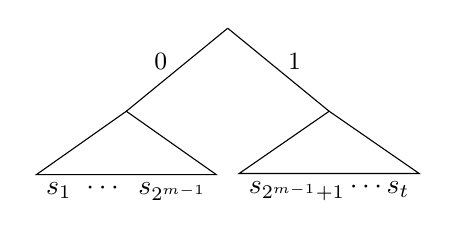
\begin{tikzpicture}
[n/.style={draw=none},
 every node/.append style={inner ysep=+0pt,outer ysep=+0pt,minimum size=+0pt}]
%\hspace{-3.9cm}
\Tree 
    [.{}
        \edge node[auto=right] {\small 0};
        \qroof{\parbox{\widthof{$s_{2^{m-1}+1}\cdots s_{t}$}}{\vspace*{.1cm}$s_1$\hfill$\cdots$\hfill$s_{2^{m-1}}$}}.{}
        \edge node[auto=left] {\small 1};
        \qroof{\parbox{\widthof{$s_{2^{m-1}+1}\cdots s_{t}$}}{\vspace*{.1cm}$s_{2^{m-1}+1}\cdots s_{t}$}}.{}
    ]
\end{tikzpicture}
\end{center}
Similarly, equation (\ref{eq-log-2}) for $\ell=m-1$ says that variables $x_{m-1,1},\ldots,x_{m-1,2^{m-2}}$ are the leaves of the subtree under the path $(b_m,b_{m-1})$. For example, if $(b_m,b_{m-1})=(1,0)$, the variables $x_{m-1,1},\ldots,x_{m-1,2^{m-2}}$ are equal to $x_{m,1}=s_{2^{m-1}+1},\ldots,\allowbreak x_{m,2^{m-2}}=s_{2^{m-1}+2^{m-2}}$, which are the leaves of the subtree under the path (1,0) as depicted below.
\begin{center}
\begin{tiny}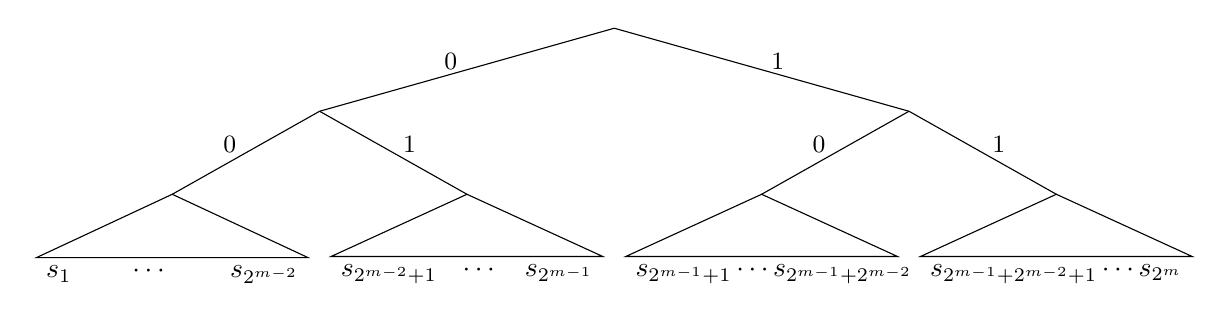
\begin{tikzpicture}
[n/.style={draw=none},
 every node/.append style={inner ysep=+0pt,outer ysep=+0pt,minimum size=+0pt}]
\Tree 
    [.{}
        \edge node[auto=right] {\small 0};
        [.{}
            \edge node[auto=right] {\small 0};
            \qroof{\parbox{\widthof{$s_{2^{m-1}+2^{m-2}+1}\cdots s_{2^{m}}$}}{\vspace*{.1cm}$s_1$\hfill$\cdots$\hfill$s_{2^{m-2}}$}}.{}
            \edge node[auto=left] {\small 1};
            \qroof{\parbox{\widthof{$s_{2^{m-1}+2^{m-2}+1}\cdots s_{2^{m}}$}}{\vspace*{.1cm}$s_{2^{m-2}+1}$\hfill$\cdots$\hfill$s_{2^{m-1}}$}}.{}
        ]
        \edge node[auto=left] {\small 1};
        [.{}
            \edge node[auto=right] {\small 0};
            \qroof{\parbox{\widthof{$s_{2^{m-1}+2^{m-2}+1}\cdots s_{2^{m}}$}}{\vspace*{.1cm}$s_{2^{m-1}+1}\cdots s_{2^{m-1}+2^{m-2}}$}}.{}
            \edge node[auto=left] {\small 1}; 
            \qroof{\parbox{\widthof{$s_{2^{m-1}+2^{m-2}+1}\cdots s_{2^{m}}$}}{\vspace*{.1cm}$s_{2^{m-1}+2^{m-2}+1}\cdots s_{2^{m}}$}}.{}
        ]
    ]
\end{tikzpicture}\end{tiny}
\end{center}

In general, the variables $x_{\ell,1},\ldots,x_{\ell,2^{\ell-1}}$ are equal to the leaves $s_{\sfleft},\ldots,\allowbreak s_{\sfright}$ under the path $(b_m,\ldots, b_\ell)$, where $\sfleft=\sum_{i=\ell}^m b_i 2^{i-1}+1$ and $\sfright=\sfleft+2^{\ell-1}-1$. 
Therefore, for $\ell=1$ equation (\ref{eq-log-2}) says that the variable $x_{1,1}$ is equal to the leaf $s_{\sfleft}=s_{\sfright}=s_\alpha$, since $\sfleft=\sfright=\sum_{i=1}^m b_i2^{i-1}+1=\alpha$, which is the unique leaf (and the unique node) in the subtree under the path $(b_m,\ldots, b_1)$.

Similarly as in Chandran et al.'s proof, for each new variable a new commitment must be added to the proof. But, in contrast with Chandran et al.'s proof, in this case the additional commitments do increase the asymptotic size of the proof. Indeed, the total number of new variables is \(2^{m-1}+2^{m-2}+\ldots+1=2^m-1=t-1\), and thus $t-1$ new commitments must be added.

One can reduce the total size of the commitments using the length reducing multi-Pedersen commitments from Section~\ref{sec:ext-mp}. However, this must be done carefully in order to be able to express equation (\ref{eq-log-2}) with a Groth-Sahai proof of an equation that involves the MP commitments and the variables $b_1,\ldots,b_m$. For example, if one computes a single commitment to all variables $\MP.\Com_{ck}((x_{1,1},\ldots,x_{m,2^{m-1}})^\top;r)$ it is not clear how to use it to express equation (\ref{eq-log-2}), because not all the variables appear at once in this equation (but all the variables appear in the previous commitment). Our solution is to compute a single MP commitment to each vector that appears in equation (\ref{eq-log-2}) in order to show with Groth-Sahai proofs that
\begin{small}
\begin{align*}
\MP.\Com_{ck_\ell}\left(
                    \pmatri{x_{\ell,1}\\\vdots\\x_{\ell,2^{\ell-1}}};r_\ell\right)
=\ &(1-b_\ell)\MP.\Com_{ck_\ell}\left(\pmatri{x_{\ell+1,1}\\\vdots\\x_{\ell+1,2^{\ell-1}}};r_{\ell,1}\right)+\\
& b_\ell\MP.\Com_{ck_\ell}\left(\pmatri{x_{\ell+1,2^{\ell-1}+1}\\\vdots\\x_{\ell+1,2^\ell}};r_{\ell,2}\right)+\\
& \MP.\Com_{ck_\ell}(\vecb{0};y_\ell),
\end{align*}
\begin{align*}
&\Longleftrightarrow\\
&\MP.\Com_{ck_\ell}\left(\begin{array}{c}
    \pmatri{x_{\ell,1}\\\vdots\\x_{\ell,2^{\ell-1}}}
    -(1-b_\ell)\pmatri{x_{\ell+1,1}\\\vdots\\x_{\ell+1,2^{\ell-1}}}
    -b_\ell\pmatri{x_{\ell+1,2^{\ell-1}+1}\\\vdots\\x_{\ell+1,2^\ell}};\\
    r_\ell-(1-b_\ell)r_{\ell,1}-b_\ell r_{\ell,2}
\end{array}\right)\\
&=
\MP.\Com_{ck_\ell}(\vecb{0};y_\ell)
\end{align*}\end{small}
for each $\ell\in[m]$ and some $y_\ell\in\Z_q$. In this way, we only need $3m=3\log t$ additional commitments. The reason for using different commitment keys for each $\ell\in[m]$ will be clear when we explain soundness.

Concretely, the prover computes
\begin{align*}
&[\vecb{c}_\ell]_1=\MP.\Com_{ck_\ell}((x_{\ell,1},\ldots,x_{\ell,2^{\ell-1}})^\top;r_\ell),\\
\end{align*}
for random $r_\ell\in\Z_q$ and $\ell\in[m]$, and 
\begin{align*}
&[\vecb{c}_{\ell,1}]_1=\MP.\Com_{ck_{\ell}}((x_{\ell+1,1},\ldots,x_{\ell+1,2^{\ell-1}})^\top;r_{\ell,1}),\\
&[\vecb{c}_{\ell,2}]_1=\MP.\Com_{ck_{\ell}}((x_{\ell+1,2^{m-1}+1},\ldots,x_{\ell+1,2^\ell})^\top;r_{\ell,2}),\\
\end{align*}
for random $r_{\ell,1},r_{\ell,2}\in\Z_q$ and $\ell\in[m-1]$. Note that the prover does not need to compute commitments to $(x_{m+1,1},\ldots,x_{m+1,t})^\top$ since $x_{m+1,i}=s_i$, $i\in[t]$, and thus they can be computed by the verifier.

Then, the prover shows that equation (\ref{eq-log-2}) holds with a GS proof of
the satisfiability of
\begin{align}
&[\vecb{c}_\ell]_1-(1-b_\ell)[\vecb{c}_{\ell,1}]_1-b_\ell[\vecb{c}_{\ell,2}]_1 = \MP.\Com_{ck_\ell}(\vecb{0};y_\ell), \text{ for } \ell \in[m],  \label{eq-log-5}
\end{align}
where $[\vecb{c}_{m,1}]:=\MP.\Com_{ck_m}((s_1,\ldots,s_{2^{m-1}})^\top;0)$ and $[\vecb{c}_{m,2}]:=\allowbreak \MP.\Com_{ck_m}(\allowbreak (s_{2^{m-1}+1},\allowbreak\ldots,s_{t})^\top;0)$ can be directly computed by the verifier, and $y_\ell:=r_\ell-(1-b_\ell)r_{\ell,1}-b_\ell r_{\ell,2}$. It also computes Groth-Sahai proofs that
\begin{equation}
b_\ell(b_\ell-1)=0 \label{eq-bit-gs}
\end{equation}
for each $\ell\in[m]$ (or equivalently a proof that $b_\ell\in\bits$).

The prover also shows that equation (\ref{eq-log-3}) is satisfied with a QA-NIZK proof that
\begin{equation}
[\vecb{c}]_1\text{ and }[\vecb{c}_1]_1\text{ open to the same value}, \label{eq-log-6}
\end{equation}
using the proof system from Section \ref{sec:aggcommit}.

Note that variables $x_{\ell+1,1},\ldots,x_{\ell+1,2^{\ell-1}}$ appear in both $[\vecb{c}_{\ell,1}]_1$ and $[\vecb{c}_{\ell+1}]_1$, as well as $x_{\ell+1,2^{\ell-1}+1},\ldots,x_{\ell+1,2^\ell}$ appear in both $[\vecb{c}_{\ell,2}]_1$ and $[\vecb{c}_{\ell+1}]_1$. To get a sound proof, the prover needs to show that this redundancy is consistent. That is, the prover needs to show that $[\vecb{c}_{\ell,1}]_1$ and $[\vecb{c}_{\ell,2}]_1$ are commitments to the first and last halves of the opening of $[\vecb{c}_{\ell+1}]_1$.

For \(\ell\in[m]\), let \(ck_\ell:=([\matr{G}_\ell]_1,\allowbreak[\vecb{g}_{\ell,2^{\ell-1}+1}]_1)\in\GG_1^{2\times{2^{\ell-1}+1}}\) the commitment key of a MP commitment scheme and let
\begin{align*}
&\matr{G}_{\ell,1}:=
\begin{pmatrix}
    \vecb{g}_{\ell,1}&\cdots&\vecb{g}_{\ell,2^{\ell-2}}
\end{pmatrix},
&\matr{G}_{\ell,2}:=
\begin{pmatrix}
    \vecb{g}_{\ell,2^{\ell-2}+1}&\cdots&\vecb{g}_{\ell,2^{\ell-1}}
\end{pmatrix}\\
&\matr{G}_\ell:=\matr{G}_{\ell,1}\cat\matr{G}_{\ell,2}
\end{align*}
To prove consistency the prover will show that, for each $\ell\in [m-1]$, the following linear system is satisfied
{\begin{align}
&\begin{pmatrix}
\vecb{c}_{\ell+1}\\
\vecb{c}_{\ell,1}\\
\vecb{c}_{\ell,2}
\end{pmatrix}
=
&\left(\begin{array}{cc|ccc}
\matr{G}_{\ell+1,1}           & \matr{G}_{\ell+1,2}            & \vecb{g}_{\ell+1,2^\ell+1} & \vecb{0}                     & \vecb{0}\\
\matr{G}_{\ell}               & \matr{0}_{2\times2^{\ell-1}}   & \vecb{0}                   & \vecb{g}_{\ell,2^{\ell-1}+1} & \vecb{0} \\
\matr{0}_{2\times 2^{\ell-1}} & \matr{G}_{\ell}                & \vecb{0}                   & \vecb{0}                     & \vecb{g}_{\ell,2^{\ell-1}+1}
\end{array}\right)
\vecb{w},\label{eq-log-split}
\end{align}}%
for some \(\vecb{w}\in\Z_q^{2^\ell+3}\), which can be proven using the proof system from Section \ref{sec:concat}.

Intuitively, \(\vecb{w}\) should be equal to \((x_{\ell+1,1},\ldots,x_{\ell+1,2^{\ell}},\allowbreak r_{\ell+1},r_{\ell,1},r_{\ell,2})\) and thus 
\begin{align*}
&[\vecb{c}_{\ell,1}]_1=\MP.\Com_{ck_\ell}(\allowbreak(x_{\ell+1,1},\ldots,x_{\ell+1,2^{\ell-1}})^\top;r_{\ell,1})\text{ and }\\
&[\vecb{c}_{\ell,2}]_1=\MP.\Com_{ck_\ell}((x_{\ell+1,2^{\ell-1}+1},\ldots, x_{\ell+1,2^{\ell}})^\top;r_{\ell,2}).
\end{align*}
However, since multi-Pedersen commitments have multiple openings it might be the case that the satisfying witness of the proof is different from \((x_{\ell+1,1},\ldots,\allowbreak x_{\ell+1,2^\ell},r_{\ell+1},r_{\ell,1},r_{\ell,2})\) and thus the intuitive reasoning is invalid.

Despite this flawed reasoning, we will show that the proof system is still sound.

\subsubsection{Soundness Intuition}
Suppose that an adversary against soundness outputs GS commitments to \(b_1,\ldots,b_{m}\in\Z_q\), outputs commitments \([\vecb{c}_\ell]_1\), $\ell\in[m]$, and \([\vecb{c}_{\ell,1}]_1,[\vecb{c}_{\ell,2}]\), $\ell\in[m-1]$, a GS proofs of the satisfiability of equation (\ref{eq-log-5}), and QA-NIZK proofs of (\ref{eq-log-6}) and (\ref{eq-log-split}) for each \(\ell\in[m-1]\).
Note that perfect soundness of Groth-Sahai proofs for equation (\ref{eq-bit-gs}) imply that \(b_1,\ldots,b_m\in\bits\).

For $\ell\in[m]$, define $\alpha_\ell$ as the position of $s_\alpha$ respective to the leaves under the path $(b_m,\ldots, b_\ell)$, that is $\alpha_\ell:=\alpha-\sfleft+1$. Note that $\alpha_\ell \in[1,2^{\ell-1}]$ since
$$
1\leq\alpha_\ell = \sum_{i=1}^m b_i2^{i-1}-\sum_{i=\ell}^mb_i2^{i-1}+1 = \sum_{i=1}^{\ell-1}b_i2^{i-1}+1\leq 2^{\ell-1}.
$$

The key observation is that, for a fixed $\alpha\in[m]$, even if in equation (\ref{eq-log-2}) $x_{\ell,j}$ is not correctly computed for $j\neq\alpha_\ell$, it holds that $x_{m,1}=s_\alpha$ anyway. We will take advantage of this observation and the fact that the adversary commits to a fixed $\alpha=\sum_{i=1}^n b_i2^{i-1}+1$ to guarantee perfect soundness of equation (\ref{eq-log-2}) at least for coordinate $\alpha_\ell$ for each $\ell\in[m]$. We do so by picking the commitment key $ck_\ell$ in such a way that its $\alpha_\ell$ th column is linearly independent from the other columns. Although we will not be able to guarantee that $x_{\ell,j}$ is correctly computed if $j\neq\alpha_\ell$, at least we will be able to do so for $x_{\ell,\alpha_\ell}$.

In the reduction we will guess the (sub-)path $(b_{m-1},\ldots, b_1)$ (it will be not necessary to guess first the edge of the path) chosen by the adversary. While in the real scheme $\mathrm{rank}(\matr{G}_\ell)=1$, for each $\ell\in[m]$, we jump to a game where $\vecb{g}_{\ell,\alpha_\ell}$ is linearly independent from the other $2^{\ell-1}$ vectors in $ck_\ell$. This can be done choosing  random $b'_{m-1},\ldots, b'_1\in\bits$ and aborting if $(b'_{m-1},\ldots, b'_{1})\neq(b_{m-1},\cdots, b_1)$. Therefore, our security reduction will have a security loss factor of $1/2^{m-1}=2/\setsize$. We sample $ck_\ell\gets\distlin_1^{2^{\ell-1},\alpha_\ell}$, as defined on Section \ref{sec:mddh}, which implies that for every $\ell\in[m]$ there exists unique $\tilde{x}_{\ell},\tilde{r}_\ell\in\Z_q$ such that $\vecb{c}_\ell:=\tilde{x}_\ell\vecb{g}_{\ell,\alpha_\ell}+\tilde{r}_\ell\vecb{g}_{\ell,2^{\ell-1}+1}$.

We prove by induction on \(\ell\) that \(\vecb{c}_\ell= s_\alpha\vecb{g}_{\ell,\alpha_\ell}+\tilde{r}_{\ell}\vecb{g}_{\ell,2^{\ell-1}+1}\), for some $\tilde{r}_\ell\in\Z_q$. If this is the case $\vecb{c}_1=s_\alpha\vecb{g}_{1,1}+\tilde{r}_{1}\vecb{g}_{1,2}$. Soundness of proof for equation (\ref{eq-log-6}) together with the fact that \(ck_1\) is perfectly binding implies that \(x=\tilde{x}_{1}=s_{\alpha}\in S\) which proves soundness.

First, it will be useful to prove the next lemma about $\alpha_\ell$.
\begin{lemma} Let $b_m,\ldots,b_1\in\bits$. For all $\ell\in[m-1]$, $\alpha_{\ell+1}=\alpha_{\ell}+b_\ell2^{\ell-1}$.
\label{lemma:alpha}
\end{lemma}
\begin{proof}
To avoid confusion, define here $\sfleft_\ell:=\sum_{i=\ell}^m b_i2^{i-1}+1$ (previously simply defined as $\sfleft$, the index of the leftmost leaf under the path $(b_m,\cdots, b_\ell)$). It holds that
\begin{align*}
\alpha_{\ell+1} &= \alpha - \sfleft_{\ell+1} + 1\\
&= \sum_{i=1}^{m} b_i2^{i-1} - \sum_{i=\ell+1}^{m}b_i2^{i-1} +1\\
&= \sum_{i=1}^{m} b_i2^{i-1} - \sum_{i=\ell}^{m}b_i2^{i-1} +1 +b_\ell2^{\ell-1}\\
&= \alpha - \sfleft_\ell +1 +b_\ell2^{\ell-1}\\
&=\alpha_\ell+b_\ell2^{\ell-1}
\end{align*}
\end{proof}

Now we prove that, for all $\ell\in[m]$, \(\vecb{c}_\ell= s_\alpha\vecb{g}_{\ell,\alpha_\ell}+\tilde{r}_{\ell}\vecb{g}_{\ell,2^{\ell-1}+1}\).
In the base case ($\ell=m$) the fact that \(\vecb{g}_{m,i}\in\Span(\vecb{g}_{m,2^{m-1}+1})\) if \(i\neq \alpha_m\) together with Lemma \ref{lemma:alpha} implies that 
\begin{align*}
\vecb{c}_m &= (1-b_m)\sum_{i=1}^{2^{m-1}}s_i \vecb{g}_{m,i}+b_m\sum_{i=1}^{2^{m-1}}s_{i+2^{m-1}}\vecb{g}_{m,i}\\
&= (1-b_m)s_{\alpha_m}\vecb{g}_{m,\alpha_m} +b_ms_{\alpha_m+2^{m-1}}\vecb{g}_{m,\alpha_m}+\tilde{r}_1\vecb{g}_{m,2^{m-1}+1}\\
&= (1-b_m)s_{\alpha-\sfleft+1}\vecb{g}_{m,\alpha_m} +b_ms_{\alpha-\sfleft+1+2^{m-1}}\vecb{g}_{m,\alpha_m}+\tilde{r}_1\vecb{g}_{m,2^{m-1}+1}\\
&=\begin{cases}
    s_{\alpha-1+1}\vecb{g}_{m,\alpha_m}+\tilde{r}_1\vecb{g}_{m,t/2} & \text{ if } b_m=0 \ (\text{and thus }\sfleft=1) \\
    s_{\alpha-(2^{m-1}+1)+1+2^{m-1}}\vecb{g}_{m,\alpha_m}+\tilde{r}_1\vecb{g}_{m,t/2} & \text{ if } b_m=1 \ (\text{and thus }\sfleft=2^{m-1}+1) 
\end{cases}
\end{align*}
for some \(\tilde{r}_1\in\Z_q\). In both cases $\vecb{c}_m=s_\alpha\vecb{g}_{1,\alpha_m}+\tilde{r}_1\vecb{g}_{m,t/2}$.

In the inductive case we assume that \(\vecb{c}_{\ell+1}=s_{\alpha}\vecb{g}_{\ell+1,\alpha_{\ell+1}}+\tilde{r}_{\ell+1}\vecb{g}_{\ell+1,2^\ell+1}\) and we want to show that $\vecb{c}_\ell = s_\alpha\vecb{g}_{\ell,\alpha_\ell}+\tilde{r}_\ell\vecb{g}_{\ell,2^{\ell-1}+1}$. Since \(\vecb{g}_{\ell+1,\alpha_{\ell+1}}\) is linearly independent from the rest of vectors in \(ck_{\ell+1}\), any solution to equation (\ref{eq-log-split}) is equal to \(s_{\alpha}\) at position \(\alpha_{\ell+1}=\alpha_\ell+b_\ell2^{\ell-1}\) as depicted below.
\begin{align*}
\pmatri{\vecb{c}_{\ell+1}\\\vecb{c}_{\ell,1}\\\vecb{c}_{\ell,2}}=
\pmatri{
\cdots & \vecb{g}_{\ell+1,\alpha_\ell} & \cdots  & \vecb{g}_{\ell+1,\alpha_\ell+2^{\ell-1}} & \cdots\\
\cdots & \vecb{g}_{\ell,\alpha_\ell}     & \cdots  & \vecb{0}                           & \cdots\\
\cdots & \vecb{0}                        & \cdots  & \vecb{g}_{\ell,\alpha_\ell}        & \cdots
}
\pmatri{\vdots\\s_\alpha\\\vdots}
\end{align*}
If $b_{\ell}=0$, by Lemma \ref{lemma:alpha}, $\alpha_{\ell+1}=\alpha_\ell$. Therefore, any solution to equation (\ref{eq-log-split}) is equal to $s_\alpha$ at position $\alpha_\ell$ and thus $\vecb{c}_{\ell,1} = s_\alpha\vecb{g}_{\ell,\alpha_\ell}+\tilde{r}_{\ell,1}\vecb{g}_{\ell,2^{\ell-1}+1}$.
Equation (\ref{eq-log-5}) implies that
\begin{align*}
\vecb{c}_{\ell}=&(1-b_\ell)(s_\alpha\vecb{g}_{\ell,\alpha_\ell}+\tilde{r}_{\ell,1}\vecb{g}_{\ell,2^{\ell-1}+1})+b_\ell\vecb{c}_{\ell,2}+y_\ell\vecb{g}_{\ell,2^{\ell-1}+1}\\
               =& s_\alpha\vecb{g}_{\ell,\alpha_\ell}+(\tilde{r}_{\ell,1}+y_\ell)\vecb{g}_{\ell,2^{\ell-1}+1}.
\end{align*}
If $b_{\ell}=1$, then $\alpha_{\ell+1}=\alpha_\ell+2^{\ell-1}$ and similarly, $\vecb{c}_{\ell}=s_\alpha\vecb{g}_{\ell,\alpha_\ell}+(\tilde{r}_{\ell,2}+y_\ell)\vecb{g}_{\ell,2^{\ell-1}+1}$.




        
%\section{Preliminaries}


\section{Our Construction}
    
	Let $\setsize:=|S|$ and \(m:=\log \setsize \). The statement is now \([\grkb{\zeta}_1]=\GS.\Com_{ck_\GS}(x_1;r_1),\ldots,\allowbreak[\grkb{\zeta}_n]_1=\GS.\Com_{ck_\GS}(x_n;r_n)\), for some $n\in\mathbb{N}$, and the prover wants to show that \(x_i=s_{\alpha_i}\), for all \(i\in[n]\) and \(\alpha_i=\sum_{j=1}^m b_{i,j}2^{j-1}+1\), for some $b_{i,1},\ldots,b_{i,m}\in\bits$. We need to reformulate equations (\ref{eq-log-2}) and (\ref{eq-log-3}) to take in count new variables. For \(\ell\in [m],i\in[n]\), define
\begin{align*}
&\vecb{x}_\ell^i:=
\begin{pmatrix}
\vecb{x}^i_{\ell,1}\\
\hline
\vecb{x}^i_{\ell,2}
\end{pmatrix}
:=
\begin{pmatrix}
x^i_{\ell,1}\\\vdots\\x^i_{\ell,2^{\ell-2}}\\
\hline
x^i_{\ell,2^{\ell-2}+1}\\\vdots\\x^i_{\ell,2^{\ell-1}}
\end{pmatrix},
&\vecb{x}^i_{m+1,1} := \begin{pmatrix}
s_1\\\vdots\\s_{t/2}
\end{pmatrix},\text{ and }
&\vecb{x}^i_{m+1,2} := \begin{pmatrix}
s_{t/2+1}\\\vdots\\s_{\setsize }
\end{pmatrix},
\end{align*}
and define new equations for each $\ell\in[m],i\in[n]$
\begin{align}
&\vecb{x}^i_\ell=({1}-{b}_{i,\ell})\vecb{x}^i_{\ell+1,1}+{b}_{i,\ell}\vecb{x}^i_{\ell+1,2},\label{eq-alog-1}\\
&x_i= \vecb{x}^{i}_1\label{eq-alog-2}
\end{align}

Next, we construct an aZKSMP for $S\subset\Z_q$ and in Section~\ref{sec:improved-aZKSMP-group-case} we show how to extend these ideas for the case of fixed \(S\subset\GG_1\).
The construction follows the intuition outlined before but it ``aggregates'' many instances on a single \(\Theta(\log \setsize )\) proof. From a high level this is done as follows.

We will rewrite equation (\ref{eq-alog-1}), which is a system of $m n$ equations, as $m$ equations of the form
\begin{equation}
\vecb{x}\vecb{y}^\top=\pmatri{
    0      & x_1y_2 & \cdots & x_1y_n\\
    x_2y_1 & 0      & \cdots & x_2y_n\\
    \vdots & \vdots & \ddots & \vdots\\
    x_my_1 & x_my_2 & \cdots & 0},
\label{eq-diag}
\end{equation}
where $\vecb{x}\in\Z_q^m,\vecb{y}\in\Z_q^n$ (i.e.~the diagonal of the matrix $\vecb{x}\vecb{y}^\top$ is $\vecb{0}$). We will use similar techniques to those of Chapter \ref{sec:bits} to give a constant size proof for the satisfiability of each of these equations. Therefore, to prove $m$ of these equations we will require $\Theta(m)=\Theta(\log t)$ group elements.

We can compute $\vecb{x}\vecb{y}^\top$ in the ``commitment space'' by means of $[\vecb{c}]_1[\vecb{d}^\top]_2$, where $[\vecb{c}]_1:=\MP.\Com_{ck_1}(\vecb{x};r_1)$ and $[\vecb{d}]_2:=\MP.\Com_{ck_2}(\vecb{y};r_2)$. Indeed, by the definition of MP commitments it holds that
\begin{align*}
[\vecb{c}]_1[\vecb{d}^\top]_2
=&\left(\sum_{i=1}^{m}x_i[\vecb{g}_i]_1+r_1[\vecb{g}_{m+1}]_1\right)\left(\sum_{j=1}^{n}y_j[\vecb{h}_j^\top]_2+r_2[\vecb{h}_{n+1}^\top]_2\right)\\
=&\sum_{i=1}^m\sum_{j=1}^n x_iy_j[\vecb{g}_i\vecb{h}_j^\top]_T+\sum_{i=1}^{m}x_ir_2[\vecb{g}_i\vecb{h}_{n+1}^\top]_T+\sum_{j=1}^{n+1}r_1y_j[\vecb{g}_{m+1}\vecb{h}_j^\top]_T
\end{align*}

Therefore, if the diagonal of $\vecb{x}\vecb{y}^\top$ is $\vecb{0}$, then $[\vecb{c}]_1[\vecb{d}^\top]_2$ is in the space spanned by $\{[\vecb{g}_i\vecb{h}_j^\top]_T:i\neq j \text{ or }i=m+1\text{ or } j=n+1\}$. Similarly as done in Section \ref{sec:bits-intuition}, equation (\ref{eq-diag}) can be proven computing two matrices $[\matr{\Theta}]_1\in\GG_1^{2\times2}$ and $[\matr{\Pi}]_2\in\GG_2^{2\times 2}$ and showing that $[\vecb{c}]_1[\vecb{d}^\top]_2=[\matr{\Theta}]_1[\matr{I}]_2+[\matr{I}]_1[\matr{\Pi}]_2$ and $\matr{\Theta}+\matr{\Pi}\in\Span(\{\vecb{g}_i\vecb{h}_j^\top:i=m+1\text{ or }j=n+1\})$.

For each $\ell\in[m]$, to rewrite the right side of equation (\ref{eq-alog-1}) in the $\vecb{x}\vecb{y}^\top$ form, we observe that
\begin{align*}
\pmatri{\vecb{x}^1_{\ell+1,1}\\\vdots\\\vecb{x}^n_{\ell+1,1}}\left(\pmatri{b_{1,\ell}\\\vdots\\b_{n,\ell}}-\pmatri{1\\\vdots\\1}\right)^\top+
\pmatri{\vecb{x}^1_{\ell+1,1}\\\vdots\\\vecb{x}^n_{\ell+1,2}}\pmatri{b_{1,\ell}\\\vdots\\b_{n,\ell}}^\top
&=\\
\begin{pmatrix}
(1-b_{1,\ell})\vecb{x}^1_{\ell+1,1}+b_{1,\ell}\vecb{x}^1_{\ell+1,2} & \cdots & (1-b_{n,\ell})\vecb{x}^1_{\ell+1,1}+b_{n,\ell}\vecb{x}^1_{\ell+1,2}\\
\vdots & \ddots  & \vdots\\ 
(1-b_{1,\ell})\vecb{x}^n_{\ell+1,1}+b_{1,\ell}\vecb{x}^n_{\ell+1,2} & \cdots & (1-b_{n,\ell})\vecb{x}^n_{\ell+1,1}+b_{n,\ell}\vecb{x}^n_{\ell+1,2}
\end{pmatrix}.&
\end{align*}
If we view the previous matrix as one of size $n\times n$ where each entry is a vector from $\Z_q^{2^{\ell-1}}$, then the diagonal forms the right side of equation (\ref{eq-alog-1}). We rewrite the left side of equation (\ref{eq-alog-1}) as
\begin{align*}
\pmatri{\vecb{x}^1_\ell\\\vdots\\\vecb{x}^n_\ell}\pmatri{1\\\vdots\\1}^\top
=
\begin{pmatrix}
\vecb{x}^1_\ell & \cdots & \vecb{x}^1_\ell\\
\vdots          &        & \vdots         \\
\vecb{x}^n_\ell & \cdots & \vecb{x}^n_\ell
\end{pmatrix}.
\end{align*}
and, again, the diagonal forms the left side of equation (\ref{eq-alog-1}). 

Now we prove that equation (\ref{eq-alog-1}) holds by replacing variables with MP commitments and showing that
\begin{align*}
[\vecb{c}_\ell]_1\left(\sum_{j=1}^n[\vecb{h}_j]_2\right)^\top-[\vecb{c}_{\ell,1}]_1\left([\vecb{d}_\ell]_2-\sum_{j=1}^n[\vecb{h}_j]_2\right)^\top-[\vecb{c}_{\ell,2}]_1[\vecb{d}]_2^\top
=&\\
[\matr{\Theta}]_1[\matr{I}]_2+[\matr{I}]_1[\matr{\Pi}]_2&,
\end{align*}
where
\begin{align*}
&[\vecb{c}_\ell]_1:=\MP.\Com_{ck_\ell}\left(\pmatri{\vecb{x}^1_\ell\\\vdots\\\vecb{x}^n_\ell};r_\ell\right)
&[\vecb{d}_\ell]_1:=\MP.\Com_{ck}\left(\pmatri{b_{1,\ell}\\\vdots\\b_{n,\ell}};t_\ell\right)\\
&[\vecb{c}_{\ell,1}]_1:=\MP.\Com_{ck_\ell}\left(\pmatri{\vecb{x}^1_{\ell+1,1}\\\vdots\\\vecb{x}^n_{\ell+1,1}};r_{\ell,1}\right)
&[\vecb{c}_{\ell,2}]_1:=\MP.\Com_{ck_\ell}\left(\pmatri{\vecb{x}^1_{\ell+1,2}\\\vdots\\\vecb{x}^n_{\ell+1,2}}\right)\\
&ck_\ell:=[\pmatri{\matr{G}_{\ell}^{1}&\cdots&\matr{G}_{\ell}^{n} & \vecb{g}_{\ell,n2^{\ell-1}+1}}]_1
&\matr{G}_{\ell}^{i}:=\pmatri{\vecb{g}_{\ell,(i-1)2^{\ell-1}+1}&\cdots&\vecb{g}_{\ell,i2^{\ell-1}}}\\
&ck:=[\matr{H}]_2 &
\matr{H}:=\pmatri{\vecb{h}_1&\cdots&\vecb{h}_n&\vecb{h}_{n+1}}.
\end{align*}
We need to show that $\matr{\Theta}+\matr{\Pi}$ is in the appropriate space, which is the one without components ``in the diagonal'' or with components in $\vecb{g}_{\ell,n2^{\ell-1}+1}\vecb{h}_j$ or $\vecb{g}_i\vecb{h}_{n+1}$ for any $i\in[n2^{\ell-1}],j\in[n+1]$. However, since we are working with matrices whose entries are vectors in $\Z_q^{2^{\ell-1}}$, we in fact need to show that
$$
\matr{\Theta}+\matr{\Pi}\in\Span(\{\vecb{g}_{\ell,i}\vecb{h}_j^\top:j\in[n+1],i\notin[(j-1)2^{\ell-1}+1,j2^{\ell-1}]\setminus[n2^{\ell-1}+1]\}),
$$
since the indices $i$ and $j$ where $i\in[(j-1)2^{\ell-1}+1,j2^{\ell-1}]$ are those which range over the elements in the diagonal of a matrix whose entries are elements from $\Z_q^{2^{\ell-1}}$.

It is only left to prove the ``aggregated version'' of equation (\ref{eq-log-split}) from the non-aggregated case,  and to prove equation (\ref{eq-alog-2}).
Equation (\ref{eq-log-split}) is proven in the same way as in the non-aggregated case, but enlarging the matrix as consequence of the enlargement of commitment keys. Additionally, we prove equation (\ref{eq-alog-2}) with a proof that
\begin{align*}
[\grkb{\zeta}_1]_1,\ldots,[\grkb{\zeta}_n]_1 \text{ and } [\vecb{c}_1]_1 \text{ open to the same values,}
\end{align*}
using the proof system from Section \ref{sec:aggcommit}.
\iffalse
We prove soundness in the same fashion as the protocols from Chapter \ref{sec:shuf-rp}, that is we guess the index $j^*$ of an element $x_{j^*}\notin S$ in order to choose $\vecb{h}_{j^*}$ linearly independent from the other vectors in $ck$. Similarly as in the non-aggregated case, we will guess the (sub-)path $(b_{j^*,m+1},\ldots, b_{j^*,1})$ (where $b_{j^*,1},\ldots,b_{j^*,m}$ are the uniques openings of, respectively, $[\vecb{d}_1]_2,\ldots,[\vecb{d}]_m$ at position $j^*$) and we will choose, for each $\ell\in[m]$, $\vecb{g}_{\ell,\alpha_{j^*,\ell}}$ linearly independent from the other vectors in $ck_\ell$, where $\alpha_{j^*,\ell}:=(\alpha_{j^*}-1 \mod 2^{\ell-1})+1$. With such choice of the commitment keys, we will be able to prove that $x_{j^*}=s_{\alpha_{j^*}}$ unless we can break some hardness assumption.
Consequently, the total security loss in the reduction will be of a factor of $\frac{2}{nt}$.  
\fi
\subsubsection{The Scheme}

\begin{description}

\item[{\(\algK_1(\gk, ck_\GS)\)}:]
Parse $ck_\GS$ as $[\vecb{u}_1\cat\vecb{u_2}]_1$.
For each \(\ell\in [m]\) let \(\matr{G}_\ell:=\matr{G}_{\ell}^{1}\cat\cdots\cat\matr{G}_{\ell}^{n}\cat\vecb{g}_{\ell,{n2^{\ell-1}+1}}\gets\distlin_1^{n2^{\ell-1}+1,0}\), where
\begin{align*}
&\matr{G}_{\ell}^{i}=
(\matr{G}_{\ell,1}^{i}|\matr{G}_{\ell,2}^{i})
=\\
&(\vecb{g}_{\ell,(i-1)2^{\ell-1}+1}\cdots\vecb{g}_{\ell, (i-1) 2^{\ell-1}+2^{\ell-2}}|\vecb{g}_{\ell,(i-1)2^{\ell-1}+2^{\ell-2}+1}\cdots\vecb{g}_{\ell,i2^{\ell-1}})
\in\Z_q^{2\times 2^{\ell-1}},
\end{align*}
 \(i\in  [n]\), and define \(ck_\ell:=[\matr{G}_\ell]_1\).
Let \(\matr{H}=\begin{pmatrix}\vecb{h}_1&\cdots&\vecb{h}_n&\vecb{h}_{n+1}\end{pmatrix}\gets\distlin_1^{n,0}\) and define \(ck:=[\matr{H}]_2\). 

For each \(\ell\in[m]\), \( i\in [n2^{\ell-1}+1]\), \(j\in  [n+1]\), such that \(i\notin [(j-1)2^{\ell-1}+1,j2^{\ell-1}]\) define matrices
\[\matr{M}^{\ell}_{i,j}:=([\matr{C}_{i,j}^{\ell}]_1,[\matr{D}_{i,j}^{\ell}]_2):=([\vecb{g}_{\ell,i}\vecb{h}_j^{\top}+\matr{T}]_1,[-\matr{T}]_2),\]
For \(\ell\in [m]\), pick \(\matr{T}\gets\Z_q^{2\times 2}\) and let
$$
\mathcal{M}_\ell:=\{\matr{M}^\ell_{i,j}:j\in[n+1],i\notin[(j-1)2^{\ell-1}+1,j2^{\ell-1}]\setminus[n2^{\ell-1}+1]\}$$
and let
$$
\mathcal{C}_\ell:=\{\matr{C}^\ell_{i,j}:j\in[n+1],i\notin[(j-1)2^{\ell-1}+1,j2^{\ell-1}]\setminus[n2^{\ell-1}+1]\}.
$$

Let \(\Pi_\sfsum\) be the proof system for sum in subspace 
(Section~\ref{sec:sum}), \(\Pi_\mathsf{lin}\) the proof system for membership in linear subspaces from Section~\ref{sect:QANIZKlinspace}, \(\Pi_\sfbits\) the proof system for proving that many commitments open to bit-strings from section \ref{sec:matr-bits}, and \(\Pi_\sfcom\)
be an instance of the proof system for equal commitment opening (Section~\ref{sec:aggcommit}).

For each $\ell\in[m]$, let
\(\crs_{\sfsum,\ell} \gets \Pi_\sfsum.\algK_1(\gk, \mathcal{M}_\ell)\).\footnote{We identify
matrices in \(\GG_1^{2 \times 2}\) (respectively in \(\GG_2^{2 \times 2}\)) with vectors in \(\GG_1^{4}\) (resp. in \(\GG_2^{4}\)).}, let \(\crs_{\mathsf{lin},\ell}\gets \Pi_\mathsf{lin}.\algK_1(gk;\allowbreak[\matr{G}_{\ell,\mathsf{split}}]_1,n2^{\ell-1}+3)\), let \(\crs_\sfbits\gets\Pi_\sfbits.\algK_1(gk,[\matr{H}]_2,m)\), and let \(\crs_\sfcom \gets \Pi_\sfcom.\algK_1(\gk, ck_1,CK_\GS,m)\), where
\begin{align*}
&\matr{G}_{\ell,\mathsf{split}}:=\\
&\begin{pmatrix}
\matr{G}^1_{\ell+1,1} & \matr{G}^{1}_{\ell+1,2} & \cdots & \matr{G}^{n}_{\ell+1,1} & \matr{G}^{n}_{\ell+1,2} & \vecb{g}_{\ell+1,n2^\ell+1} & \matr{0}                       & \matr{0}\\
\matr{G}^{1}_{\ell,1}   & \matr{0}              & \cdots & \matr{G}^n_{\ell,n}   & \matr{0}              & \matr{0}                  & \vecb{g}_{\ell,n2^{\ell-1}+1}  & \matr{0}\\
\matr{0}              & \matr{G}^1_{\ell,1}   & \cdots & \matr{0}              & \matr{G}^n_{\ell,n}   & \matr{0}                  & \matr{0}                       & \vecb{g}_{\ell,n2^{\ell-1}+1}
\end{pmatrix},\\
&CK_\GS:=\pmatri{
    [\vecb{u}_1]_1 &        & [\vecb{0}]_1   & [\vecb{u}_2]_1 &        & [\vecb{0}]_1\\
               & \ddots &            &            & \ddots &         \\
    [\vecb{0}]_1   &        & [\vecb{u}_1]_1 & [\vecb{0}]_1   &        & [\vecb{u}_2]_1
}\in\GG_1^{2n\times2n}.
\end{align*}
The common reference string is given by:
\begin{eqnarray*}
\mathsf{crs}&:=&\left( gk, [\matr{G}]_1,
    [\matr{H}]_2, \{\mathcal{M}_\ell,\crs_{\sfsum,\ell},\crs_{\mathsf{lin},\ell}:\ell\in [m]\},\crs_\sfbits,\crs_\sfcom \right).
 \end{eqnarray*}


\item[{\(\algP(\mathsf{crs}, ([\grkb{\zeta}_1]_1, \ldots, [\grkb{\zeta}_n]_1,S), \langle (x_1,\ldots,x_n),(w_1,\ldots,w_n) \rangle)\)}:]
The prover compute commitments
\begin{align*}
&[\vecb{c}_\ell]_1:=\MP.\Com_{ck_\ell}({\vecb{x}_\ell^1}^\top,\ldots,{\vecb{x}_\ell^n}^\top;r_\ell), \text{ for } \ell \in [m],\\
&[\vecb{c}_{\ell,1}]_1:=\MP.\Com_{ck_\ell}({\vecb{x}^1_{\ell+1,1}}^\top,\ldots,{\vecb{x}^n_{\ell+1,1}}^\top;r_{\ell,1}),\\
&[\vecb{c}_{\ell,2}]_1:=\MP.\Com_{ck_\ell}({\vecb{x}^1_{\ell+1,2}}^\top,\ldots,{\vecb{x}^n_{\ell+1,2}}^\top;r_{\ell,2}), \text{ for } \ell\in[m-1]\\
&[\vecb{d}_\ell]_2:=\MP.\Com_{ck}(\vecb{b}_\ell;t_\ell),\text{ for } \ell\in[m]
\end{align*}
 where \(r_\ell,r_{\ell,1},r_{\ell,2},t_j\gets\Z_q\) and the variables \(\vecb{x}^i_\ell,\vecb{x}^i_{\ell,j},\vecb{b}_\ell\) are the ones defined in equation (\ref{eq-alog-1}). The prover computes a proof \(\pi_\sfbits\) that \([\vecb{d}_1]_2,\ldots,[\vecb{d}_m]_2\) open to bit-strings. Then, for \(\ell\in [m]\), the prover pick matrices \(\matr{R}_\ell\gets\Z_q^{2\times 2}\), computes
\begin{align*}
&([\matr{\Theta}_\ell]_1,[\matr{\Pi}_\ell]_2)  := \\
&\quad \sum_{i=1}^n\sum_{j\neq i}\sum_{k=1}^{2^{\ell-1}}(x^i_{\ell,k}-x^i_{\ell+1,k}(1-b_{j,\ell})-x^i_{\ell+1,2^{\ell-1}+k}b_{j,\ell})\matr{M}_{(i-1)2^{\ell-1}+k,j}^{\ell}\\
&\quad+ \sum_{i=1}^n\sum_{k=1}^{2^{\ell-1}}t_\ell(x^i_{\ell+1,k}-x^i_{\ell+1,2^{\ell-1}+k})\matr{M}_{(i-1)2^{\ell-1}+k,n+1}^{\ell} \\
&\quad+ \sum_{j=1}^n (r_\ell-r_{\ell,1}(1-b_{j,\ell})-r_{\ell,2}b_{j,\ell})\matr{M}_{n2^{\ell-1}+1,j}^{\ell} \\
&\quad+(r_{\ell,1}-r_{\ell,2})t_\ell\matr{M}^{\ell}_{n2^{\ell-1}+1,n+1}+([\matr{R}_\ell]_1,[-\matr{R}_\ell]_2),
\end{align*}
where \(r_{1,1}=r_{1,2}=0\), and computes proofs $\pi_{\mathsf{lin},\ell},\pi_{\mathsf{sum},\ell}$ that, respectively,
\begin{align*}
&\begin{pmatrix}
\vecb{c}_{\ell+1}\\\vecb{c}_{\ell,1}\\\vecb{c}_{\ell,2}
\end{pmatrix}\in
\Span(\matr{G}_{\ell,\mathsf{split}})\ (\text{ if }\ell< m), &\matr{\Theta_\ell}+\matr{\Pi_\ell}\in\Span(\mathcal{C}_\ell).
\end{align*}
Finally, it computes a proof \(\pi_\sfcom\) that \(([\grkb{\zeta}_1]_1,\ldots,[\grkb{\zeta}_n]_1)\) and \([\vecb{c}_1]_1\) open to the same value.

The proof is \(\pi:=(\{([\vecb{c}_\ell]_1,[\vecb{c}_{\ell,1}]_1,[\vecb{c}_{\ell,2}]_1,[\vecb{d}_\ell]_2,[\matr{\Theta}_\ell]_1,[\matr{\Pi}_\ell]_2,\pi_{\mathsf{lin},\ell},\pi_{\sfsum,\ell}):\ell\in [m]\},\pi_\sfbits,\pi_\sfcom)\).

\item[{\(\algV(\crs,([\grkb{\zeta}_1]_1, \ldots, [\grkb{\zeta}_n]_1,S),\pi)\)}:]
Let \([\vecb{c}_{m,1}]_1:=\MP.\Com_{ck_m}(s_1,\ldots,s_{\setsize /2};0),[\vecb{c}_{m,2}]:=\MP.\Com_{ck_m}(s_{\setsize /2+1},\ldots,s_{\setsize };0)\). The verifier checks the validity of \(\pi_\sfbits,\pi_\sfcom\) 
and, for each \(\ell\in [m]\), checks the validity of \(\pi_{\mathsf{lin},\ell},\pi_{\sfsum,\ell}\) and of equations
\begin{align}
&[\vecb{c}_\ell]_1\left(\sum_{j=1}^n [\vecb{h}_j]_2\right)^\top-
[\vecb{c}_{\ell,1}]_1\left(\sum_{j=1}^n[\vecb{h}_j]_2-[\vecb{d}_\ell]_2\right)^\top-
[\vecb{c}_{\ell,2}]_1[\vecb{d}_\ell]_2^\top = \nonumber\\
&[\matr{\Theta}_\ell]_1[\matr{I}]_2+[\matr{I}]_1[\matr{\Pi}_\ell]_2. \label{eq-alog-5}
\end{align}
If any of these checks fails, it rejects the proof.

\item[{\(\mathsf{S}_1({gk},ck_\GS)\):}] The simulator receives as input a description of an asymmetric bilinear group \({gk}\) and a GS commitment key $ck_\GS$. It generates and outputs the CRS in the same way as \(\algK_1\), but additionally outputs the simulation trapdoor 
\(\tau:=(\matr{H},\tau_\sfcom,\tau_\sfbits,\{\tau_{\sfsum,\ell},\tau_{\mathsf{lin},\ell}:\ell\in [m]\})\),
where \(\tau_{\sfsum},\tau_{\sfbits},\tau_{\sfsum,\ell},\tau_{\mathsf{lin,\ell}}\) are, respectively, \({\Pi_\sfsum},{\Pi_\sfcom},\Pi_\sfsum,\Pi_\mathsf{lin}\) simulation trapdoors.

\item[{\(\mathsf{S}_2(\crs,([\grkb{\zeta}_1]_1,\ldots,[\grkb{\zeta}_n]_1,S),\tau)\):}] Define \(\vecb{x}_\ell^i:=\vecb{0}\) and \(\vecb{b}_\ell:=\vecb{0}\) for all \(\ell\in [m],i\in[n]\), and computes \([\vecb{c}_\ell]_1, [\vecb{c}_{\ell,1}]_1,[\vecb{c}_{\ell,2}]_1,[\vecb{d}_\ell]_2\) and \([\matr{\Theta}_\ell]_1,[\matr{\Pi}_\ell]_2\), as an honest prover would do (that is, with all variables set to 0).
Finally, simulate proofs \(\pi_\sfcom,\pi_\sfbits,\pi_{\sfsum,\ell},\pi_{\mathsf{lin},\ell}\) using the respective trapdoors.
\end{description}

We prove the following Theorem.

\begin{theorem} \label{theo:bits}
The proof system described above is a QA-NIZK proof system for the language \(\Lang_{ck_\GS,\mathsf{set}}^n\)
 with perfect completeness, computational soundness, and perfect zero-knowledge.
\end{theorem}	

\subsubsection{Completeness}
Completeness follows from completeness of \(\Pi_\sfsum,\Pi_\mathsf{lin},\Pi_\sfbits,\Pi_\sfcom\), and from the fact that equation (\ref{eq-alog-5}) is satisfied for each \(\ell\in [m]\):
\begin{align*}
&\vecb{c}_\ell\left(\sum_{j=1}^n \vecb{h}_j\right)^\top-
\vecb{c}_{\ell,1}\left(\sum_{j=1}^n\vecb{h}_j-\vecb{d}_\ell\right)^\top-
\vecb{c}_{\ell,2}\vecb{d}_\ell^\top &= \\
&\sum_{i=1}^n\sum_{j=1}^n\matr{G}_{\ell}^{i}\vecb{x}^i_{\ell}\vecb{h}_j^\top+\sum_{j=1}^nr_\ell\vecb{g}_{\ell,n2^{\ell-1}+1}\vecb{h}_j^\top
-\sum_{i=1}^n\sum_{j=1}^n\matr{G}_{\ell}^{i}\vecb{x}^i_{\ell+1,1}(1-b_{j,\ell})\vecb{h}_j^\top\\
&+\sum_{i=1}^n\matr{G}_{\ell}^{i}\vecb{x}^i_{\ell+1,1} t_\ell\vecb{h}_{n+1}^\top-\sum_{j=1}^nr_{\ell,1}(1-b_{j,\ell})\vecb{g}_{\ell,n2^{\ell-1}+1}\vecb{h}_j^\top+ r_{\ell,1}t_\ell\vecb{g}_{\ell,n2^{\ell-1}+1}\vecb{h}_{n+1}^\top\\
&-\sum_{i=1}^n\sum_{j=1}^n\matr{G}_{\ell}^{i}\vecb{x}^i_{\ell+1,2}b_{j,\ell}\vecb{h}_j^\top-\sum_{i=1}^n\matr{G}_{\ell}^{i}\vecb{x}^i_{\ell+1,2} t_\ell\vecb{h}_{n+1}^\top-\sum_{j=1}^nr_{\ell,2}b_{j,\ell}\vecb{g}_{\ell,n2^{\ell-1}+1}\vecb{h}_j^\top\\
&- r_{\ell,2}t_\ell\vecb{g}_{\ell,n2^{\ell-1}+1}\vecb{h}_{n+1}^\top &=\\
&\sum_{i=1}^n\sum_{j\neq i}\matr{G}_{\ell}^{i}(\vecb{x}^i_\ell-\vecb{x}^i_{\ell+1,1}(1-b_{j,\ell})-\vecb{x}^i_{\ell+1,2}b_{j,\ell})\vecb{h}_j^\top+\\
&\sum_{i=1}^n\matr{G}_{\ell}^{i}(\vecb{x}^i_{\ell+1,1}-\vecb{x}^i_{\ell+1,2})t_\ell\vecb{h}_{n+1}^\top+\sum_{j=1}^n(r_\ell-r_{\ell,1}(1-b_{j,\ell})-r_{\ell,2}b_{j,\ell})\vecb{g}_{\ell,n2^{\ell-1}+1}\vecb{h}_{j}^\top\\
&+(r_{\ell,1}-r_{\ell,2})t_\ell\vecb{g}_{\ell,n2^{\ell-1}+1}\vecb{h}_{n+1}^\top &=\\
&\sum_{i=1}^n\sum_{j\neq i}\sum_{k=1}^{2^{\ell-1}}(x^i_{\ell,k}-x^i_{\ell+1,k}(1-b_{j,\ell})-x^i_{\ell+1,2^{\ell-1}+k}b_{j,\ell}))\vecb{g}_{\ell,(i-1)2^{\ell-1}+k}\vecb{h}_j^\top\\
&+\sum_{i=1}^n\sum_{k=1}^{2^{\ell-1}}t_\ell(x^i_{\ell+1,k}-x^i_{\ell+1,2^{\ell-1}+k}\vecb{g}_{\ell,(i-1)2^{\ell-1}+k}\vecb{h}_{n+1}^\top\\
&\sum_{j=1}^n(r_\ell-r_{\ell,1}(1-b_{j,\ell})-r_{\ell,2}b_{j,\ell})\vecb{g}_{\ell,n2^{\ell-1}+1}\vecb{h}_{j}^\top+(r_{\ell,1}-r_{\ell,2})t_\ell\vecb{g}_{\ell,n2^{\ell-1}+1}\vecb{h}_{n+1}^\top &=\\
&\matr{\Theta}\matr{I}+\matr{I}\matr{\Pi}.
\end{align*}

\subsubsection{Soundness}

The following theorem guarantees soundness. 
 
\begin{theorem} Let \(\mathsf{Adv}_{{\Pi_\sfset}}(\advA)\) 
be the advantage of an adversary \(\advA\) against the soundness of 
the proof system  described above. There exist PPT adversaries
\(\advD_1,\advD_2,\advB_\sfbits,\advB_\sfcom,\advB_\sfsum,\advB_\mathsf{lin}\) such that 
\begin{align*}
\mathsf{Adv}_{{\Pi_\sfset}}(\advA) \leq 
n \left(\right.
    &\mathsf{Adv}_{\mathcal{L}_1,\Gr}(\advD_1) 
        + \setsize /2\left(4/q
            +  \mathsf{Adv}_{\Pi_\sfbits}(\advB_\sfbits)
            +  \mathsf{Adv}_{\mathcal{L}_1,\Hr}(\advB_2)\right. \\
    &+ \left.\left.\mathsf{Adv}_{{\Pi_\sfcom}}(\advB_\sfcom)
        + m\mathsf{Adv}_{{\Pi_\sfsum}}(\advB_\sfsum)
        + m\mathsf{Adv}_{{\Pi_\mathsf{lin}}}(\advB_\mathsf{lin})\right)\right).
\end{align*}
\label{teo:bitstr-soundness}
\end{theorem}

Recall that, given $b_1,\ldots,b_m\in\bits$, we defined $\alpha:=\sum_{i=1}^mb_i2^{i-1}+1$. Recall also that, given a path $(b_m,\ldots, b_\ell)$ in the binary tree whose leaves are labeled from left to right by $s_1,\ldots,s_t$, we defined $\sfleft:=\sum_{i=\ell}^m b_i2^{i-1}+1$, $\sfright:=\sfleft+2^{\ell-1}-1$, and we defined $\alpha_\ell:=\alpha-\sfleft+1$ the position of $s_\alpha$ relative to the leaves under $s_\sfleft,\ldots,s_\sfright$.

The proof follows from the indistinguishability of the following games:
\begin{itemize}
\item[\(\mathsf{Real}\):] This is the real soundness game. The output is 1 if the adversary submits some \(([\grkb{\zeta}_1]_1,\ldots,[\grkb{\zeta}_n]_1,S)\notin\Lang_{ck_\GS,\mathsf{set}}^n\) and the corresponding proof which is accepted by the verifier.
\item[\(\sfGame_0\):] This identical to \(\mathsf{Real}\), except that \(\algK_1\) does not receive \(ck_\GS\) as a input but
it samples \(ck_\GS\) itself together with its discrete logarithms.
\item[\(\sfGame_1\):] This game is identical to \(\sfGame_0\) except that now it chooses random \(j^*\in[n]\) and it aborts if \(x_{j^*}\notin S\).
\item[\(\sfGame_2\):] This game is identical to \(\sfGame_1\) except that now \(\matr{H}\gets\distlin^{n,j^*}_1\).
\item[\(\sfGame_3\):] This game is identical to \(\sfGame_2\) except that now it defines $b_m:=b_{j^*,m}$ and chooses a random (sub-)path $(b_{m-1},\cdots, b_1)\gets\bits^{m-1}$ (which ignores the first edge) in the tree whose leaves are $s_1,\ldots,s_t$. This game aborts if \((b_{j^*,1},\ldots,b_{j^*,m})\notin\bits^m\) or \((b_1,\ldots, b_{m-1})\neq(b_{j^*,1},\ldots, b_{j^*,m-1})\), where \(b_{j^*,1},\ldots,b_{j^*,m}\) are the openings of \([\vecb{d}_2]_2,\ldots,[\vecb{d}_m]_2\) at coordinate \(j^*\), respectively.
\item[\(\sfGame_4\):] This game is identical to \(\sfGame_3\) except that now \(\matr{G}_\ell\gets\distlin_1^{n2^{\ell-1},\Delta+\alpha_\ell}\), for \(\ell\in [m]\) and $\Delta:=(j^*-1)2^{\ell-1}$.
\end{itemize}

It is obvious that the first two games are indistinguishable. The rest of the argument goes as follows.

\begin{lemma}
\(\Pr\left[ \mathsf{Game}_1(\advA)=1\right]\geq\dfrac{1}{n}\Pr\left[\mathsf{Game}_0(\advA)=1\right].\)
\end{lemma}

\begin{proof}  The probability that
 \(\mathsf{Game}_1(\advA)=1\) is the probability that  a) \(\mathsf{Game}_0(\advA)=1\) and
b)  \(x_{j^*} \notin S\). The view of adversary \(\advA\) is independent of \(j^*\), while, if \(\mathsf{Game_0}(\advA)=1\), then there is at least one index \(j \in [n]\) such that  
such that  \(x_{j} \notin S\). Thus, 
the probability that the event described in b) occurs conditioned on \(\mathsf{Game_0}(\advA)=1\), is greater than or equal to \(1/n\) and the lemma follows.
\end{proof}

\begin{lemma} There exists a\ \(\distlin_1\)-\(\mddh_{\GG_2}\) adversary \(\advD_2\) such that
\(|\Pr\left[\allowbreak\mathsf{Game}_{1}(\advA)\allowbreak=1\right]\linebreak-\Pr\left[\mathsf{Game}_{2}(\advA)=1\right]|\) \(\leq \mathsf{Adv}_{\distlin_1,\ggen_a}(\advD_2).\)
\end{lemma}
\begin{proof}
We construct an adversary \(\advD_2\) that receives 
a challenge \(([\vecb{a}]_2,[\vecb{u}]_2)\) of the 
\(\distlin_1\)-\(\mddh_{\GG_2}\) assumption. From this challenge, \(\advD_2\) just defines the matrix  \([\matr{H}]_2\in\GG_2^{2\times(n+1)}\) as the matrix whose last column is \([\vecb{a}]_2\), the ith column is \([\vecb{u}]_2\), and the rest of the columns are random vectors in the image of \([\vecb{a}]_2\). 
Obviously, when \([\vecb{u}]_2\) is sampled from 
the image of \([\vecb{a}]_2,\) \(\matr{H}\) follows the distribution \(\distlinizeroone\), while if \([\vecb{u}]_2\) is a uniform element of \(\GG^2_2\), \(\matr{H}\) follows the distribution \(\distlin_1^{n,j^*}\). 
 
Adversary \(\advD_2\) samples
\(\matr{G}^{\ell} \gets \distlin_1^{n2^{\ell-1},0}\). Given that \(\advD_2\) does not know the discrete logarithms of \([\matr{H}]_2\), it cannot compute the pairs \((\matr{C}^\ell_{i,j},\matr{D}^\ell_{i,j})\) exactly as in \(\sfGame_0\). Nevertheless, for each \(\ell\in[m],i\in[n2^{\ell-1}+1],j\in[n+1]\) such that $i\notin[(j-1)2^{\ell-1}+1,j2^{\ell-1}]$, it can compute identically distributed pairs by picking \(\matr{T}\gets\Z_q^{2\times 2}\) and defining
\[
([\matr{C}^\ell_{i,j}]_1,[\matr{D}^\ell_{i,j}]_2):=([\matr{T}]_1,\vecb{g}_{\ell,i}[\vecb{h}_j]_2^\top-[\matr{T}]_2).
\]

The rest of the elements of the CRS are honestly computed. When \(\matr{H}\gets\distlin_1^{n,0}\), \(\advD_2\) perfectly simulates \(\sfGame_0\), and when \(\matr{H}\gets\distlin_1^{n,j^*}\), \(\advD_2\) perfectly simulates \(\sfGame_1\), which concludes the proof. 
\end{proof}

\begin{lemma} There exists an adversary \(\advB_\sfbits\) against \(\Pi_\sfbits\) such that
\(\Pr\left[\allowbreak \mathsf{Game}_2(\advA)\allowbreak =1\right]\geq\dfrac{2}{\setsize }(\Pr\left[\mathsf{Game}_3(\advA)=1\right]+\adv_{\Pi_\sfbits}(\advB_\sfbits)).\)
\end{lemma}

\begin{proof}  The probability that
 \(\mathsf{Game}_3(\advA)=1\) is the probability that  a) \(\mathsf{Game}_2(\advA)=1\) and
b) \((b_{j^*,1},\ldots,b_{j^*,m})\notin\bits^m\) or \((b_1,\ldots, b_{m-1}) \neq (b_{j^*,1},\ldots, b_{j^*,m-1})\). If \((b_{j^*,1},\ldots,\allowbreak b_{j^*,m})\notin\bits^m\) we can build an adversary \(\advB_\sfbits\) against \(\Pi_\sfbits\) and thus, the probability that \((b_{j^*,1},\ldots,b_{j^*,m})\in\bits^m\) is less than \(\adv_{\Pi_\sfbits}(\advB_1)\). The view of adversary \(\advA\) is independent of \((b_{1},\ldots, b_{m-1})\), while, if \(\mathsf{Game_2}(\advA)=1\) and \((b_{j^*,1},\ldots,b_{j^*,m})\in\bits^{m}\), then \((b_{j^*,1}\cdots b_{j^*,m-1})\in\bits^{m-1}\). Thus, 
the probability that the event described in b) occurs conditioned on \(\mathsf{Game_2}(\advA)=1\) and \((b_{j^*,1},\ldots,b_{j^*,m})\in\bits^{m}\), is greater than or equal to \(2/\setsize \) and the lemma follows.
\end{proof}

\begin{lemma} There exists a \(\distlin_1\)-\(\mddh_{\GG_1}\) adversary \(\advD_1\) such that
\(|\Pr\left[\mathsf{Game}_{3}(\advA)=1\right]\allowbreak-\Pr\left[\mathsf{Game}_{4}(\advA)=1\right]|\) $\leq
    \mathsf{Adv}_{\distlin_1,\GG_1}(\advD_1).$
\label{lemma:bits2}
\end{lemma}

\begin{proof}
We construct an adversary \(\advD_1\) that receives 
a challenge \(([\vecb{a}]_1,[\vecb{u}]_1)\) of the 
\(\distlin_1\)-\(\mddh_{\GG_1}\) assumption. From this challenge, \(\advD_1\) defines for each \(\ell\in [m]\) the matrix  \([\matr{G}_\ell]_1\) as the matrix whose  \(\Delta+\alpha_\ell\) th column is \([\vecb{u}]_1\), and the rest of the columns are random vectors in the image of \([\vecb{a}]_1\). 
Obviously, when \([\vecb{u}]_1\) is sampled from 
the image of \([\vecb{a}]_1\), \([\matr{G}_\ell]_1\) follows the distribution \(\distlin_1^{n2^{\ell-1},0}\), while if \([\vecb{u}]_1\) is a uniform element of \(\GG^2_1\), \([\matr{G}_\ell]_1\) follows the distribution \(\distlin_1^{n2^{\ell-1},\Delta+\alpha_\ell}\). 
 
The rest of the elements of the CRS are honestly computed. When \([\vecb{u}]_1\) is sampled from the image of \([\matr{a}]_1\), \(\advD_1\) perfectly simulates \(\sfGame_3\), and when \([\vecb{u}]_1\) is uniform, \(\advD_1\) perfectly simulates \(\sfGame_4\), which concludes the proof. 
\end{proof}


\begin{lemma}
There exist adversaries \(\advB_\sfcom\), against the strong soundness of \(\Pi_\sfcom\), \(\advB_\sfsum\), against the soundness of \(\Pi_\sfsum\), and an adversary \(\advB_\mathsf{lin}\) against the soundness of \(\Pi_\mathsf{lin}\), such that \(\Pr[\sfGame_4(\advA)=1]\leq 4/q+ \adv_{\Pi_\sfcom}(\advB_\sfcom)+m\adv_{\Pi_\sfsum}(\advB_\sfsum)+m\adv_{\Pi_\mathsf{lin}}(\advB_\mathsf{lin})\).
\end{lemma}
\begin{proof}
With probability \(1-4/q\), \(\{\vecb{g}_{\ell,\Delta+\alpha_\ell},\vecb{g}_{\ell,n2^{\ell-1}+1}\}\), \(\ell\in [m]\), and \(\{\vecb{h}_{j^*},\allowbreak \vecb{h}_{m+1}\}\) are bases of \(\Z_q^2\),
and, for each \(\ell\in [m],\mu\in\{1,2\}\), we can define \(\tilde{s}_\ell,\tilde{s}_{\ell,\mu},\tilde{r}_\ell,\tilde{r}_{\ell,\mu},b_{j^*,\ell},\tilde{t}_\ell\) as the unique coefficients in \(\Z_q\) such that \(\vecb{c}_\ell=\allowbreak \tilde{s}_\ell\vecb{g}_{\ell,\Delta+\alpha_\ell} + \tilde{r}_\ell \vecb{g}_{\ell,n2^{\ell-1}+1}, \vecb{c}_{\ell,\mu}=\tilde{s}_{\ell,\mu}\vecb{g}_{\ell,\Delta+\alpha_\ell} + \tilde{r}_{\ell,\mu} \vecb{g}_{\ell,n2^{\ell-1}+1},\) and \(\vecb{d}_\ell= b_{j^*,\ell} \vecb{h}_{j^*} + \tilde{t}_\ell \vecb{h}_{n+1}\).

Recall that if \(\sfGame_4(\advA)=1\) then \(x_{j^*}\notin S\). The adversary can win in \(\sfGame_4\) if one of the following events happen:
\begin{description}
\item[\(E_1\):] the adversary breaks soundness of \(\Pi_\sfcom\) and \(x_{j^*}\neq \tilde{s}_1\),
\item[\(E_2\):] the adversary breaks one of the \(m\)  instances of \(\Pi_\sfsum\) and \(\matr{\Theta}_\ell+\matr{\Pi}_\ell\notin\Span(\mathcal{C}_\ell)\),
\item[\(E_3\):] the adversary breaks one of the \(m\) instances of \(\Pi_\sflin\) and \((\vecb{c}_{\ell+1},\vecb{c}_{\ell,1},\vecb{c}_{\ell,2})\notin\Span(\matr{G}_{\ell,\mathsf{split}})\),
\item[\(E_4\):] neither of \(E_1\),\(E_2\), or \(E_3\) happens, but \(x_{j^*}\notin S\) anyway.
\end{description}
By the law of total probabilities, \(\Pr[\sfGame_4(\advA)=1]\leq 4/q+\Pr[E_1]+\Pr[E_2]+\Pr[E_3]+\Pr[E_4]\), and is not hard to see that there exist adversaries \(\advB_\sfcom,\advB_\sfsum,\advB_\mathsf{lin}\) such that \(\Pr[E_1]=\adv_{\Pi_\sfcom}(\advB_\sfcom),\Pr[E_2]=m\adv_{\Pi_\sfsum}(\advB_\sfsum),\) and \(\Pr[E_3]=m\adv_{\Pi_\mathsf{lin}}(\advB_\mathsf{lin})\). Below we will show that \(\Pr[E_4]=0\) (using the same argument used in the non-aggregated case).

We prove by induction on \(\ell\) that \(\tilde{s}_\ell=s_{\alpha}\). If this is the case, the fact that \(\neg E_1\) implies that \(x_{j^*}=\tilde{s}_1=s_{\alpha}\in S\), which finish the proof.

But first note that given a vector \(\vecb{k}\in\Z_q^2\), such that \(\vecb{h}_j^\top\vecb{k}=1\) if \(j=j^*\) and \(0\) if not (which exists since \(\{\vecb{h}_{j^*},\vecb{h}_{n+1}\}\) is a basis of \(\Z_q^2\)), if we multiply equation (\ref{eq-alog-5}) on the right by $\vecb{k}$ we get
$$
[\vecb{c}_\ell]_T-(1-b_{j^*,\ell})[\vecb{c}_{\ell,1}]_T-b_{j^*,\ell}[\vecb{c}_{\ell,2}]_T=[(\matr{\Theta}_\ell+\matr{\Pi}_\ell)\vecb{k}]_T.
$$
The fact that \(\matr{\Theta}_\ell+\matr{\Pi}_\ell\in\Span(\mathcal{C}_\ell)\), \(\vecb{g}_{\ell,i}\in\Span(\vecb{g}_{\ell,n2^{\ell-1}+1})\) if \(i\neq \Delta+\alpha_\ell\), and $\Delta+\alpha_\ell\in[\Delta+1,\Delta+2^{\ell-1}]$, implies that
$$(\matr{\Theta}_\ell+\matr{\Pi}_\ell)\vecb{k} = \sum_{i\in[n2^{\ell-1}+1]\setminus[\Delta+1,\Delta+2^{\ell-1}]}\beta_i\vecb{g}_{\ell,i}=\beta\vecb{g}_{\ell,n2^{\ell-1}+1}$$
for some $\beta_i,{\beta}\in\Z_q$, $i\in[n2^{\ell-1}+1]\setminus[\Delta+1,\Delta+2^{\ell-1}]$.

Therefore, given that we are in the case $b_\ell=b_{j^*,\ell}$, equation (\ref{eq-alog-5}) implies that
$$
[\vecb{c}_\ell]_T=(1-b_{\ell})[\vecb{c}_{\ell,1}]_T+b_{\ell}[\vecb{c}_{\ell,2}]_T+\beta\vecb{g}_{\ell,n2^{\ell-1}+1}.
$$

In the base case ($\ell=m$), the fact that \(\vecb{g}_{m,i}\in\Span(\vecb{g}_{m,n2^{m-1}+1})\), if \(i\neq \Delta+\alpha_m\), implies that 
\begin{align*}
\vecb{c}_m &= (1-b_m)\sum_{i=1}^{2^{m-1}}s_i \vecb{g}_{m,\Delta+i}+b_m\sum_{i=1}^{2^{m-1}}s_{i+2^{m-1}}\vecb{g}_{m,\Delta+i}\\
&= (1-b_m)s_{\alpha_m}\vecb{g}_{m,\Delta+\alpha_m} +b_ms_{\alpha_m+2^{m-1}}\vecb{g}_{m,\Delta+\alpha_m}+\tilde{r}_1\vecb{g}_{m,n2^{m-1}+1}\\
&= (1-b_m)s_{\alpha-\sfleft+1}\vecb{g}_{m,\Delta+\alpha_m} +b_ms_{\alpha-\sfleft+1+2^{m-1}}\vecb{g}_{m,\Delta+\alpha_m}+\tilde{r}_1\vecb{g}_{m,n2^{m-1}+1}\\
&=\begin{cases}
    s_{\alpha-1+1}\vecb{g}_{m,\Delta+\alpha_m}+\tilde{r}_1\vecb{g}_{m,n2^{m-1}+1} & \text{ if } b_m=0 \ (\sfleft=1) \\
    s_{\alpha-(2^{m-1}+1)+1+2^{m-1}}\vecb{g}_{m,\Delta+\alpha_m}+\tilde{r}_1\vecb{g}_{m,n2^{m-1}+1} & \text{ if } b_m=1 \ (\sfleft=2^{m-1}+1) 
\end{cases}
\end{align*}
for some \(\tilde{r}_1\in\Z_q\). In both cases $\vecb{c}_1=s_\alpha\vecb{g}_{m,\Delta+\alpha_m}+\tilde{r}_1\vecb{g}_{m,n2^{m-1}}$.

In the inductive case we assume that \(\vecb{c}_{\ell+1}=s_{\alpha}\vecb{g}_{\ell+1,2\Delta+\alpha_{\ell+1}}+\tilde{r}_{\ell+1}\vecb{g}_{\ell+1,n2^\ell+1}\) and we want to show that $\vecb{c}_\ell = s_\alpha\vecb{g}_{\ell,\Delta+\alpha_\ell}+\tilde{r}_\ell\vecb{g}_{\ell,n2^{\ell-1}+1}$.\footnote{Note that $\matr{G}_{\ell+1}\gets\distlin_1^{n2^\ell, (j^*-1)2^\ell+\alpha_{\ell+1}}$ and thus, the $(j^*-1)2^\ell+\alpha_{\ell+1}=2\Delta+\alpha_{\ell+1}$ th column of $\matr{G}_{\ell+1}$ is l.i.~from the rest.} Since \(\vecb{g}_{\ell+1,\alpha_{\ell+1}}\) is linearly independent from the rest of vectors in \(ck_{\ell+1}\), any solution to 
\begin{equation}
\begin{pmatrix}\vecb{c}_{\ell+1}\\\vecb{c}_{\ell,1}\\\vecb{c}_{\ell,2}\end{pmatrix}=\matr{G}_{\ell,\mathsf{split}}\vecb{w} \label{eq-G-split}
\end{equation}
is equal to \(s_{\alpha}\) at position \(2\Delta+\alpha_{\ell+1}=2\Delta+\alpha_\ell+b_\ell2^{\ell-1}\) as depicted below.
\begin{align*}
\pmatri{\vecb{c}_{\ell+1}\\\vecb{c}_{\ell,1}\\\vecb{c}_{\ell,2}}=
\pmatri{
\cdots & \vecb{g}_{\ell+1,2\Delta+\alpha_\ell} & \cdots  & \vecb{g}_{\ell+1,2\Delta+\alpha_\ell+2^{\ell-1}} & \cdots\\
\cdots & \vecb{g}_{\ell,\Delta+\alpha_\ell}     & \cdots  & \vecb{0}                           & \cdots\\
\cdots & \vecb{0}                        & \cdots  & \vecb{g}_{\ell,\Delta+\alpha_\ell}        & \cdots
}
\pmatri{\vdots\\s_\alpha\\\vdots}
\end{align*}
If $b_{\ell}=0$, by Lemma \ref{lemma:alpha}, $\alpha_{\ell+1}=\alpha_\ell$. Therefore, any solution to equation (\ref{eq-G-split})
 is equal to $s_\alpha$ at position $2\Delta+\alpha_\ell$ and thus $\vecb{c}_{\ell,1} = s_\alpha\vecb{g}_{\ell,\Delta+\alpha_\ell}+\tilde{r}_{\ell,1}\vecb{g}_{\ell,n2^{\ell-1}+1}$.
Equation \ref{eq-alog-5} implies that
\begin{align*}
\vecb{c}_{\ell}=&(1-b_\ell)(s_\alpha\vecb{g}_{\ell,\Delta+\alpha_\ell}+\tilde{r}_{\ell,1}\vecb{g}_{\ell,n2^{\ell-1}+1})+b_\ell\vecb{c}_{\ell,2}+y_\ell\vecb{g}_{\ell,n2^{\ell-1}+1}\\
               =& s_\alpha\vecb{g}_{\ell,\Delta+\alpha_\ell}+(\tilde{r}_{\ell,1}+y_\ell)\vecb{g}_{\ell,n2^{\ell-1}+1}.
\end{align*}
If $b_{\ell}=1$, then $\alpha_{\ell+1}=\alpha_\ell+2^{\ell-1}$ and similarly, $\vecb{c}_{\ell}=s_\alpha\vecb{g}_{\ell,\Delta+\alpha_\ell}+(\tilde{r}_{\ell,2}+y_\ell)\vecb{g}_{\ell,n2^{\ell-1}+1}$.

\end{proof}
\subsubsection{Perfect Zero-Knowledge}
Note that the vectors \([\vecb{c}_\ell],[\vecb{c}_{\ell,1}]_1,[\vecb{c}_{\ell,2}]_1,[\vecb{d}_\ell]_2\) and matrices \([\matr{\Theta}_\ell]_1,[\matr{\Pi}_\ell]_2\), \(1\leq\ell\leq m\), output by the prover and the simulator are, respectively, uniform vectors and uniform matrices conditioned on satisfying equation \ref{eq-alog-5}. This follows from the fact that \(ck,ck_1,\ldots,ck_\ell\) are all perfectly hiding commitment keys and that \([\matr{\Theta}_\ell]_1,[\matr{\Pi}_\ell]_1\) are the unique solutions of equation (\ref{eq-alog-5}) modulo the random choice of \(\matr{R}_\ell\). Finally, the rest of the proof follows from zero-knowledge of \(\Pi_\sfcom,\Pi_\sfbits,\Pi_\sfsum,\) and \(\Pi_\mathsf{lin}\).

\subsection{The case \(S\subset\GG_1\)} \label{sec:improved-aZKSMP-group-case}
We briefly justify that the case \(S\subset\GG_1\) follows directly from the case \(S\subset\Z_q\) when \(S\) is a fixed witness samplable set. That is, there is a fixed set $S$ for each CRS, and there is an efficient algorithm that samples \(s_1,\ldots,s_{\setsize }\in\Z_q\) such that \(S=\{[s_1]_1,\ldots,[s_{\setsize }]_1\}\). %Note that this is the same case of Section~\ref{sec:bits-applications} where the CRS depends on set.

The reason why is not clear how to compute proofs in this setting is that it requires to compute values of the type \([\vecb{s}_i \gamma]_1\), where \([\gamma]_\mu\), \(\mu\in\{1,2\}\), is a group element included in the CRS. The solution is straightforward: use \(s_1,\ldots,s_{\setsize }\) to compute these values and add them to the CRS (with the consequent CRS growth). Therefore, the new CRS contains also, for each $\alpha\in[n],\ell\in[m],i\in[n2^{\ell-1}],j\in[n]$, such that $i\neq(j-1)2^{\ell-1}+\alpha_\ell$:
\begin{align*}
s_\alpha[\vecb{g}_{\ell,(i-1)2^{\ell-1}+\alpha_\ell}]_1 \text{ and }
 s_\alpha([\matr{C}^\ell_{(i-1)2^{\ell-1}+\alpha_\ell,j}]_1,[\matr{D}_{(j-1)2^{\ell-1},j}^\ell]_2).
\end{align*}




\bibliographystyle{alpha}
\bibliography{cryptobib/abbrev2,cryptobib/crypto,manualbib}
\end{document}

